\documentclass[11pt,a4paper,twoside,openright]{report}

\usepackage{graphicx}
\usepackage{tabularx}
\usepackage{afterpage}
\usepackage{amsmath,amssymb}
\usepackage{bm}
\usepackage{float}
\usepackage{mathtools}
\usepackage{rotating}
\usepackage{fancyhdr}
\usepackage[figurewithin=none]{caption}
\usepackage[font=small]{caption}
%\usepackage[scriptsize]{caption}
%\usepackage{subcaption}
\usepackage{algpseudocode}
\usepackage{algorithm}
\usepackage{subfigure}
\usepackage{hyperref}
\usepackage[space]{grffile} 
\usepackage{color}
\usepackage{placeins}
\usepackage{breqn}
\usepackage{systeme}
\usepackage{amssymb,amsmath}
\setlength{\oddsidemargin} {2. cm}
\setlength{\evensidemargin} {2. cm}
\addtolength{\oddsidemargin} {-0.4 cm}
\addtolength{\evensidemargin} {-0.4 cm}
\linespread{1.1}


\usepackage[english]{babel}

\usepackage[utf8]{inputenc}


\usepackage{url}

\pagestyle{empty}

\begin{document}
\thispagestyle{empty}
\vspace*{-1.5cm}
 \bfseries{
\begin{center}
  \large
  POLITECNICO DI MILANO\\
  \normalsize
  Computer Science and Engineering Master Degree\\
  Dipartimento di Elettronica Informazione e Bioingegneria\\
  \begin{figure}[htbp]
    \begin{center}
      
\includegraphics[width=3.5cm]{./img/logo/logo poli}
    \end{center}
  \end{figure}
  \vspace*{0.1cm} \LARGE


  \textbf{TITOLO DELLA TESI}\\


  \vspace*{.75truecm} \large
 %  \vspace*{0.5truecm} \large
  Artificial Intelligence and Robotic Laboratory \newline of Politecnico di Milano
\end{center}
\vspace*{2.0cm} \large
%\vspace*{2.0cm} \large
\begin{flushleft}


  Supervisor: Prof. Marcello Restelli \\

  \begin{tabbing}  
      Co-supervisors: Alessandro Lavelli, Dott.

  \end{tabbing}
\end{flushleft}
\vspace*{1.0cm}
%\vspace*{0.5cm}
\begin{flushright}


  Master thesis of:\\ Nome Cognome Matricola\\


\end{flushright}
\vspace*{0.8cm}
\begin{center}

  Academic Year 2018-2019
\end{center} \clearpage
}

\thispagestyle{empty} \normalfont \cleardoublepage
\thispagestyle{empty}  \cleardoublepage
\pagenumbering{Roman}
\newpage
\chapter*{Abstract}

\addcontentsline{toc}{chapter}{Abstract}

This work studies the design and development of an autonomous agent in the context of racing games using Reinforcement Learning. As the Reinforcement Learning techniques have progressed throughout the years more successful agents have been developed in games scenarios. 
Our work aims at finding the best trajectory on a specific race track in the Open Race Car Simular (TORCS), a racing simulator that throughout the years has become the standard software for academic research.
We focused on two different approaches of RL algorithms.
The former involves trying to follow and improve a human demonstration trajectory within a single task.
The latter adopts a two-step approach, consisting in: first, trying to follow the human demonstration trajectory as better as possible. Then, upon on that, trying to improve the lap-time.
After our trials we stated that the second approach is more successful, and we will show the experimental results to prove that.
\newpage
\chapter*{Sommario}

\addcontentsline{toc}{chapter}{Sommario}

TESTO DEL SOMMARIO
%\thispagestyle{empty} \vspace*{.75truecm} \cleardoublepage
%\include{chapters/acknowledgements}
\thispagestyle{empty} \vspace*{.75truecm} \normalfont \cleardoublepage
\pagestyle{plain}\renewcommand{\chaptermark}[1]{\markboth{\chaptername\ \thechapter.\ #1}{}}
\renewcommand{\sectionmark}[1]{\markright{\thesection.\ #1}}
\fancyhead[LE,RO]{\bfseries\thepage}
   
\fancyhead[RE]{\bfseries\leftmark} 
\fancyhead[LO]{\bfseries\rightmark}   
\renewcommand{\headrulewidth}{0.3pt}

%\pagenumbering{arabic}
\setcounter{tocdepth}{3}
\setcounter{secnumdepth}{3}

\tableofcontents

\listoffigures

\listoftables

\chapter{Introduction}
\label{Introduction}
\thispagestyle{empty}
\pagenumbering{arabic}

In the last decade autonomous driving has been deeply studied in several fields of research: automotive, military, racing cars, and even flight. The goal is to disrupt the need of a human driver or pilot, resulting in a reduction in costs and an increase of safety, for instance by reducing the number of accidents per year due to human error. Moreover, they could learn from their errors, and transmit to each other autonomous vehicle instantaneously, so that each of them is constantly up to date.
However, researches in the area of autonomous driving traces back to the birth of the first computers. In the '40, the scientific community were trying and gain insight about the human mind, in order to build artificial agents that could replicate -or even outperform- human in some specific tasks.
That's how computer science branched into paths such as artificial intelligence and robotics.
One of the main goal of the research of artificial intelligence has always been autonomous driving, that is the capability for an agent of perceiving the world and moving accordingly in order to reach a specific target.
Autonomous cars consists in some piece of hardware capable of moving, such as a traditional car, or a drone, equipped with some sensors give insight on the environment, one or more computer units whith a decision making algorithm, which compute an action to perform by means of some actuators, such as a throttle, a break, a steering, or a transmission.
One of the first experiments in embodying some intelligence in an artificial agent were William Grey Walter's Turtle Robots in the '50s. They were capable of moving in the sorroundings by sensing the environment in a simplified manner. They consisted in front wheel drive tricycle-like robots covered by a clear plastic shell, and were provided with a photocell and a bump detector as sensors, which resulted in the action of a motor. Despite their simple behaviors, the technique Walter used are reflected in today's reactive and biologically-inspired robots such as those based on the B.E.A.M philosophy.
Later on, in 1989, a new tentative of building an autonomous car was ALVINN, which stands for Autonomous Land Vehicle In a Neural Network, developed for military research.
At that time the technology was not sophisticated enough to provide the computation required to drive in real time, but in a sense the premise of the algorithm used nowadays was already there. In fact, neural networks are today the essential tools for building an autonomous car.
Later on with the advent of more and more sophisticated electronic components, such as sensors (Lidars and Radars, which are capable of scanning the environment at 360 degree via electromagnetic waves), and with the continuous improvement of electronic components, such as GPUs, autonomous driving started being a hot topic in industry beside scientific research.
In the last decade, some of the traditional automotive companies, such as BMW, Mercedes-Benz, General Motors, Audi, started investing in this reasearch providing their cars with a multitude of sensors and algorithms to make their cars autonomous. Ford is another manufacturer with deployments already in play, with self-driving vehicles being tested in Pittsburgh, Palo Alto, Miami, Washington D.C. and Detroit, with Austin, Texas joining them soon. Together with its partner Argo AI, Ford has plans to trial its fleet of self-driving cars in Austin with a view towards launching a wider-reaching autonomous taxi and delivery service in 2021.
Tesla, one of the companies founded by Elon Musk, is also making big steps forward in taking autonomy into mainstream use, both in terms of real world use cases and potential monetization of self-driving technologies. Tesla has supplied customers with more than 780,000 vehicles since launching, the majority of which arrive with pre-installed, self-driving capabilities available to users who purchase the requisite software. Tesla autonomous vehicles have logged huge levels of miles driven since their introduction, growing from 0.1 billion miles in May 2016 to an estimated 1.88 billion miles as of October 2019.
Waymo, the newborn firm from Google's Alfabet, has been carrying out successful trials of autonomous taxis in California, transporting over 6,200 people in the first month and many thousands since. They're proving a practical business case for autonomous vehicles.
Also in the U.S., Walmart is using autonomous cargo vans to deliver groceries in Arizona, while Pizza Hut is working with Toyota on a driverless electric delivery vehicle that even has a mobile kitchen in it to cook pizzas en route to your house.
Parallely, in the military field, DARPA (Defense Advanced Research Projects Agency) has been proposing every year since 2007 a challenge called DARPA Grand Challenge, in which scientist teams dare each other to reach some targets as fast as possible.
The reasons for this race to the autonomous driving are millions of possible accidents avoided per year, and a reduction of pollution and costs by sharing cars which are capable of transporting people without human intervention needed. %nel caso si può ampliare% 
This growth in the reaserach on autonomous cars led to a formalization of the levels of automation: Society of Automotive Engineers (SAE) introduced six levels of automation: level 0 is no automation, that is traditional cars we are accustomed to. With Level 1, driver assistance, relating to computer assistance of simple driving functions like the cruise control or automated braking systems. Cruise control consists in the capability of mantaining a certain target speed, whatever the slope of the road, weather condition, asphalt roughness. It can be accomplished via some speed sensors and a PID controller, there is no need of complex artificial intelligence. Automated braking systems involves stopping the car or reducing the speed whenever an object come across, be it a vehicle or a pedestrian. It requires proximity and distance sensors (ultrasonic or laser sensors) and may follow some manual rules based on thresholds. Lane Crossing Alert makes the car capable of notify whenever it crosses another lane, and can be achieved with camera sensors.
Level 2 refers to partial automation, where the vehicle assists drivers with steering or acceleration, allowing drivers to disengage from some tasks.  For example instance , Adaptive Cruise Control, Lane Keeping, or self-parking.
Level 3 concerns conditional automation, where the vehicle takes over some of the monitoring of the environment from the driver, using sensor technology like LiDAR. That's what the company Tesla is currently developing: their cars are able of moving in the surroundings but the human intervention is still required in dangerous situations.
Level 4 is high automation, where much greater control has been handed to the vehicle, which is in charge of steering, braking, accelerating, monitoring the vehicle and roads, and also responding to events like deciding when to change lanes, turn or use signals.
Level 5 is full automation. No company is currently able to reach this level of automation.
Currently, most of the cars are embodied with level 1 or 2. However, level 3 and 4 are still object of research, especially by tech companies such as Tesla and Waymo, whose promise is to reach these levels of automation in ten years, and level 5 in twenty, enabling their cars with the power of fully replacing human drivers.
The reasons why today full autonomous driving has not being implemented yet are the extremely huge amount of data required for perceiving the complex world of the urban scenario and for computing the consequent actions. In fact, in order to be able to perform this vast computations, several computers and GPUs are needed aboard on the car, resulting in cost, weight, and power consumption. This is the strategy adopted by Tesla so far, whose cars to day span from a price of 85000 dollars to 120000 dollars, and weigh about 2000kg. 
Another approach, adopted by companies such as Google, is to perform computation on remote servers in their datacenters. However, current mobile connections such as 4G, makes impractical the transmission of data provided each second by the vast amount of sensors.
In the future, the advent of 5G could be a game changer in this sense, which should provide a larger in bandwidth and more stable internet connection.
That's why the scientific community is starting downstepping the complexity of the task, trying to build autonomous agents in a closed and controlled environment. This lead to a simplification of the problem, avoiding the need of a real time mapping of the environment, and excluding unattended events such as pedestrian coming across.
Whether it's a matter of hardware or software, today such goal is still out of reach. Rather, some firms are focusing their attention on making a car which is autonomous in a specifing task. For example, good results have been achieved in keeping a lane on a highway, or stopping with a pedestrian coming across. 
Alternatively, good or complete levels of autonomy could be achieved in , where the perception part could be performed by simple sensors such as gps and odometry sensors.
An example could be a race track, such as Formula 1 tracks, where the environment is known apriori, and that's where our thesis move into.
In this paper we will tackle the problem of following a trajectory driven beforehand by a human driver on a race car and, if possible, to improve it.

\chapter{Context}
\label{Context}
\thispagestyle{empty}

TESTO CAPITOLO 2

\chapter{Problem Statement}
\label{Problem_Statement}
\thispagestyle{empty}

In this chapter we provide a mathematical formulation of the problem we tackle in this thesis.
In the first part of this chapter, we define the environment as a Markov Decision Process (MDP).
As said before, the problem of designing an agent able to perform a race on track with human-like skills can be divided into two sub goals. The first is purely based on imitation learning, where the agent learns to follow the reference trajectory, whilst in the second goal a new agent is built upon the previous one and learns to improve the imitating policy.


\section{Environment Formulation}

The racing of a car on the track can be represented as an MDP, where the state corresponds to the situation of the car on the track, $\boldsymbol s \in \mathbb{R}^n,$ where $n$ is the number of features that we will define in chapter \ref{Methods}; the action $\boldsymbol a \in \mathbb{R}^3$ is a vector of three continuous variables, defined as: steering with $ a_s \in [-1,1] $, where positive values mean steer left while negative ones mean steer right, throttle with $ a_t \in [0,1] $ and brake with $ a_b \in [0,1] $. These ranges of values are given by the environment. We assume the MDP to be deterministic such that the transition probability distribution is  $p(\boldsymbol s_{t+1}=\boldsymbol s|\boldsymbol a_t, \boldsymbol s_t) = \delta(\boldsymbol s - f(\boldsymbol a_t,\boldsymbol s_t)),$ where $\delta(\boldsymbol s)$ is the Dirac Delta function and $f(\cdot)$ is a function implemented by the simulator. Thus, the transition function is embedded in the simulator.
The MDP has one starting start $S_0$ but has many terminal states. The terminal state is the final state of the episode. In our case, two situations can occur: the car reaches the endline of the track, which is considered as a success, receiving a reward of $0$ or the car goes out of track, which is considered as failure and the agent receives a negative reward signal. For intermediate steps the reward is given by a \textit{reward function} $r(\cdot),$ which will be defined in Section \ref{sec:reward_function}.
We represent the expert demonstrations as a set $\mathcal{D}=\{\boldsymbol l_i|i= 0,..,m\}$ where $m$ is the number of sampled trajectories from this MDP and $\boldsymbol l_i$ is a sequence of states and actions $\boldsymbol s_0^i,\boldsymbol a_0^i,\boldsymbol s_1^i,\boldsymbol a_1^i,...,\boldsymbol s^i_{n_i}$, where $\boldsymbol s^i_{n_i}$. It is important to note that the time-lengths of these trajectories are known.
We have access to the environment through observations $\boldsymbol x \in X$, where $\boldsymbol x$ is a vector of features that we will define in \ref{sec:obs}.

Then, we define a \textit{reference trajectory} $\boldsymbol l_{ref}$ as the shortest sequence of state-action belonging to $\mathcal{D}$, i.e. the one with the shortest time.
The reward function $r(\cdot)$ is expressed in terms of the reference trajectory. When the agent performs worse than the expert it receives a negative reward signal, whereas when it does better it receives a positive one.

\section{Reference Trajectory Following}
\label{ref_follow}

In the imitation learning problem, the parametric policy $\psi_{\boldsymbol \omega}$, with parameter vector $\boldsymbol \omega$, seeks to minimize the difference between the agent trajectory and the human demonstration. The trajectory divergence is defined as:

\begin{equation}\mathcal{L}_\tau = \frac{1}{|\tau|} \sum_{s \in \tau} {\lVert}{s - l_\perp}{\rVert}^2, \end{equation} where $\tau$ is the trajectory, $|\tau| = n$ is the trajectory length and $l_\perp$ is the projection of the state on the reference trajectory.

However, this loss is not used directly for the optimization of the policy (indeed, it does not depend on $\boldsymbol \omega$) but it is implicit in the policy $\psi_{\boldsymbol \omega}$, with parameters vector $\theta$. Therefore, the rules of the policy are parametrized by $\boldsymbol \omega$ and are expressed so as to minimize $\mathcal{L}_\tau.$ The goal of the problem, thus, is to find the parameter vector $\boldsymbol \omega$ that allows the agent to perform a lap on the track that minimizes $\mathcal{L}_\tau$. Finding the optimal $\boldsymbol \omega^*$ can be cast to an RL policy optimization problem in which the objective function to maximize is the expected return obtained by following 
\begin{equation}J(\boldsymbol \omega)=\int_{\mathcal{T}} p(\tau|\boldsymbol \omega)R(\tau)d \tau,\end{equation}
where $p(\tau|\boldsymbol \omega)$ is the trajectory density function and $R(\tau)$ is the reward of the trajectory $\tau$.

Note that by using a reward function consistent with the reference trajectory, the maximization of $J(\boldsymbol \omega)$ implicitly leads to the minimization of $\mathcal{L}_\tau.$
However, the policy $\psi_{\boldsymbol \omega}$, by design cannot perform better than the expert demonstration. For this reason, the policy $\psi_{\boldsymbol \omega}$ will be used as a base for the next step.







\section{Reference Trajectory Improvement}
\label{ref_improve}

Once the first goal is achieved, the imitating policy $\psi_{\boldsymbol \omega^*}$ is kept fixed. Upon this, a new agent is built. The goal of this second policy $\pi_{\boldsymbol{\theta}}$ is to improve the performance, i.e., the lap-time, by correcting the behaviours of the former policy. The objective function

\begin{equation}J(\boldsymbol \theta)=\int_{\mathcal{T}} p(\tau|\boldsymbol \theta)R(\tau)d \tau\end{equation}

corresponds to the expected return obtained by following the policy $\pi_{\boldsymbol{\theta}}$. The maximization of $J(\boldsymbol \theta)$, through RL policy optimization, results in finding the optimal policy parameter $\boldsymbol \theta^*$. 


Fig.\ref{fig:diagram3} is a schematic representation of the interactions between the policy $\pi_{\boldsymbol{\theta}}$, the environment and the optimized imitating policy $\psi_{\boldsymbol \omega^*}$.

The environment, after receiving an action $A_{t-1}$, gives back the observation $X_t$. Some of the features which compose $X_t$ will be useful to the imitating policy, whilst others to the improving policy. For this reason, $X_t$ is split into two vectors $X_t^{\psi}$ and $X_t^{\pi}$: the former is given as input to the imitating policy, while the latter is processed from a feature extractor $f_e$ which receives the observation and produces a vector of features $\Phi_t$, i.e., $f_e(X_t^{\pi})= \Phi_t.$
The imitating policy computes an action $A_t^{\psi_{\boldsymbol \omega^*}}$ aimed at following the reference trajectory.
Then, by combining the features $\Phi_t$ with the action $A_t^{\psi_{\boldsymbol \omega^*}}$, a new state $S_t$ is produced.
The improving policy $\pi_{\boldsymbol{\theta}}$ receives the state $S_{t+1}$ and computes a correction, or delta action $A_{t+1}^{\pi_{\boldsymbol{\theta}}}$ that, combined with $A_{t+1}^{\psi_{\boldsymbol \omega^*}}$, produces the final action $A_{t+1}$.


\begin{figure}
    \centering
 	  \captionsetup{width=10cm}
      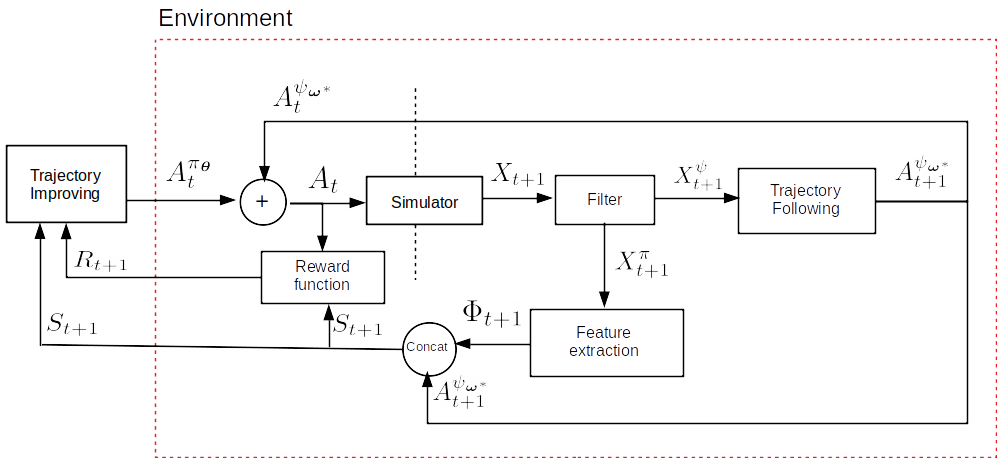
\includegraphics[width=14cm]{./img/diagram_new}
     \caption{Improving Policy, imitating Policy and Environment interface. The dashed line stands for a time step advance}
   \label{fig:diagram3}
  \end{figure}
\chapter{State of the Art}
\label{State of the Art}
\thispagestyle{empty}



Gli algoritmi di guida autonoma esistono già, c'è questo quello quell'altro
	Prima parte: 
		guida autonoma
	Seconda parte:
		Reinforcement learning based self driving car
		Videogiochi guida autonoma
		ieee transaction on ai games
		check evolutionary intelligent gaming
		gameconf
		papers su pagina di lanzi
		
- Introduzione intelligenza artificiale:
	cos'è l'intelligenza artificiale
	perchè l'intelligenza artificiale
	robots
	autonomous vehicles
	
- Autonomous vehicles
	taxonomy
	albori
		rules
	oggi
		machine learning
			reinforcement learning
				fisico (tesla, google..)
				virtuale (videogiochi)
				 
	
	











Simulators: Voyage Deep Drive, CARLA, AWS Deep Racer, Deep Traffic





			


with the dramatic improvement in hardware and the availability of a huge amount of data machine learning and deep learning techniques could have been applied to this scenario. 
In particular, reinforcement learning has been demonstrated to be quite promising for this context.







\cite{playingforbenchmarks}






Introduzione al capitolo


The objective of this chapter is to illustrate more in detail the context in which our thesis is located.
In particular, the chapter is divided in two sections. First, it describes the work done by the scientific community in the field of autonomous driving, focusing expecially on reinforcement learning based algorithms.
In the second part we provide an overview of the world of autonomous driving videogames and simulators.





Introduzione alla guida autonoma

In the last decade autonomous driving has been deeply studied in several fields of research: automotive, military, racing cars, and even fly. The goal is to disrupt the need of a human driver or pilot, resulting in a reduction in costs and an increase of safety, for instance by reducing the number of accidents per year due to human error. Moreover, they could learn from their errors, and transmit to each other autonomous vehicle instantaneously, so that each of them is constantly up to date.
Researches for autonomous driving traces back to the birth of the first computers, in the '40s. At that moment, the scientific community were trying and gain insight about the human mind, in order to build artificial agents that could replicate -or even outperform- human in some specific tasks.
That's how computer science branched into paths such as artificial intelligence and robotics.
One of the main goal of the research of artificial intelligence has always been autonomous driving, that is the capability for an agent of perceiving the world and moving accordingly in order to reach a specific target.
Autonomous cars consists in some piece of hardware capable of moving, such as a traditional car, or a drone, equipped with some sensors give insight on the environment, one or more computer units whith a decision making algorithm, which compute an action to perform by means of some actuators, such as a throttle, a break, a steering, or a transmission.
One of the first experiments in embodying some intelligence in an artificial agent were William Grey Walter's Turtle Robots in the '50s. They were capable of moving in the sorroundings by sensing the environment in a simplified manner. They consisted in front wheel drive tricycle-like robots covered by a clear plastic shell, and were provided with a photocell and a bump detector as sensors, which resulted in the action of a motor. Despite their simple behaviors, the technique Walter used are reflected in today's reactive and biologically-inspired robots such as those based on the B.E.A.M philosophy.
Later on, in 1989, a new tentative of building an autonomous car was ALVINN, which stands for Autonomous Land Vehicle In a Neural Network, developed for military research.
At that time the technology was not sophisticated enough to provide the computation required to drive in real time, but in a sense the premise of the algorithm used nowadays was already there. In fact, neural networks are today the essential tools for building an autonomous car.
Later on with the advent of more and more sophisticated electronic components, such as sensors (Lidars and Radars, which are capable of scanning the environment at 360 degree via electromagnetic waves), and with the continuous improvement of electronic components, such as GPUs, autonomous driving started being a hot topic in industry beside scientific research.
In the last decade, most of the traditional automotive companies, expecially Mercedes-Benz, Volkswagen, Volvo, started investing in this reasearch providing their cars with a multitude of sensors and algorithms to make their cars autonomous. Ford is another manufacturer with deployments already in play, with self-driving vehicles being tested in Pittsburgh, Palo Alto, Miami, Washington D.C. and Detroit, with Austin, Texas joining them soon. Together with its partner Argo AI, Ford has plans to trial its fleet of self-driving cars in Austin with a view towards launching a wider-reaching autonomous taxi and delivery service in 2021.
Tesla, one of the companies founded by Elon Musk, is also making big steps forward in taking autonomy into mainstream use, both in terms of real world use cases and potential monetization of self-driving technologies. Tesla has supplied customers with more than 780,000 vehicles since launching, the majority of which arrive with pre-installed, self-driving capabilities available to users who purchase the requisite software. Tesla autonomous vehicles have logged huge levels of miles driven since their introduction, growing from 0.1 billion miles in May 2016 to an estimated 1.88 billion miles as of October 2019.
Waymo, the newborn firm from Google's Alfabet, has been carrying out successful trials of autonomous taxis in California, transporting over 6,200 people in the first month and many thousands since. They're proving a practical business case for autonomous vehicles.
Also in the U.S., Walmart is using autonomous cargo vans to deliver groceries in Arizona, while Pizza Hut is working with Toyota on a driverless electric delivery vehicle that even has a mobile kitchen in it to cook pizzas en route to your house.
Parallely, in the military field, DARPA (Defense Advanced Research Projects Agency) has been proposing every year since 2007 a challenge called DARPA Grand Challenge, in which scientist teams dare each other to reach some targets as fast as possible.
The reasons for this race to the autonomous driving are millions of possible accidents avoided per year, and a reduction of pollution and costs by sharing cars which are capable of transporting people without human intervention needed.
This growth in the reaserach on autonomous cars led to a formalization of the levels of automation: Society of Automotive Engineers (SAE) introduced five levels of automation: with Level 1, driver assistance, relating to computer assistance of simple driving functions like the cruise control or automated braking systems. Cruise control consists in the capability of mantaining a certain target speed, whatever the slope of the road, weather condition, asphalt roughness. It can be accomplished via some speed sensors and a PID controller, there is no need of complex artificial intelligence. Automated braking systems involves stopping the car or reducing the speed whenever an object come across, be it a vehicle or a pedestrian. It requires proximity and distance sensors (ultrasonic or laser sensors) and may follow some manual rules based on thresholds. Lane Crossing Alert makes the car capable of notify whenever it crosses another lane, and can be achieved with camera sensors.
Level 2 refers to partial automation, where the vehicle assists drivers with steering or acceleration, allowing drivers to disengage from some tasks.  For example instance , Adaptive Cruise Control and Lane Keeping.
Level 3 concerns conditional automation, where the vehicle takes over some of the monitoring of the environment from the driver, using sensor technology like LiDAR. That's what the company Tesla is currently developing: their cars are able of moving in the surroundings but the human intervention is still required in dangerous situations.
Level 4 is high automation, where much greater control has been handed to the vehicle, which is in charge of steering, braking, accelerating, monitoring the vehicle and roads, and also responding to events like deciding when to change lanes, turn or use signals.
Level 5 is full automation. No company is currently able to reach this level of automation.
Currently, most of the cars are embodied with level 1 or 2. However, level 3 and 4 are still object of research, especially by tech companies such as Tesla and Waymo, whose promise is to reach these levels of automation in ten years, and level 5 in twenty, enabling their cars with the power of fully replacing human drivers.
The reasons why today full autonomous driving has not being implemented yet are the extremely huge amount of data required for perceiving the complex world of the urban scenario and for computing the consequent actions. In fact, in order to be able to perform this vast computations, several computers and GPUs are needed aboard on the car, resulting in cost, weight, and power consumption. This is the strategy adopted by Tesla so far, whose cars to day span from a price of 85000 dollars to 120000 dollars, and weigh about 2000kg. 
Another approach, adopted by companies such as Google, is to perform computation on remote servers in their datacenters. However, current mobile connections such as 4G, makes impractical the transmission of data provided each second by the vast amount of sensors.
In the future, the advent of 5G could be a game changer in this sense, which should provide a larger in bandwidth and more stable internet connection.
That's why the scientific community is starting downstepping the complexity of the task, trying to build autonomous agents in a closed and controlled environment. This lead to a simplification of the problem, avoiding the need of a real time mapping of the environment, and excluding unattended events such as pedestrian coming across.
Whether it's a matter of hardware or software, today such goal is still out of reach. Rather, some firms are focusing their attention on making a car which is autonomous in a specifing task. For example, good results have been achieved in keeping a lane on a highway, or stopping with a pedestrian coming across. 
Alternatively, good or complete levels of autonomy could be achieved in , where the perception part could be performed by simple sensors such as gps and odometry sensors.
An example could be --> agganciarsi con la notra tesi



In this paper we will tackle the problem of following a trajectory driven beforehand by a human driver on a race car and, if possible, to improve it.


	- 5 su ambienti controllati: piste formula 1 per test, videogiochi -> nostra tesi
	
	
Come si fa la guida autonoma

Automation to this level is a rather complex task: it requires a part of perception of the environment, a part of planning through an algorithm, and a part of control, to perform the actions by means of physical actuators.
- Perception:
	
	- image segmentation
	- mapping
	- odometry
	- slam
	- deep learning
	- 3d object recostruction
	- computer vision
	- sensor fusion kalman filter
	
				- hardware: lidar, gps, odometry, radar
			- software: vision, segmentation, deep learning, thresholding ecc
- Planning:
	- reinforcement learning
	- inverse reinforcement learning
	- 			- hardware: computer, gpu, 5G
			- software: 
				- reinforcement learning: policy, reward ecc
					- papers sul reinforcement learning applicati alle macchine
In our thesis we focused our attention on the planning part. In fact, by the help of a driving simulator, we could gather data with help of virtual sensors, and control the car by virtual actuators.



.Reinforcement learning autonomous driving:
	- cenni a rl e perchè è suitable a questa applicazione:
			- mondo non noto a priori
			- impara sempre
			- impara ad adattarsi
	- cosa è stato fatto
		- 
- This paper https://arxiv.org/pdf/1909.12153.pdf shows an example of end-to-end reinforcement learning application to autonomous drive, using a proximal policy optimization algorithms by means of a neural network which maps the state to the controls. - It learns two different policies: the driver and the stopper, and the reward is the squared proximity to a target position.
In this paper $https://web.stanford.edu/~anayebi/projects/CS_239_Final_Project_Writeup.pdf$ they experiment different setups of Deep Neural Networks, such as CNN and RNN as functions approximator of a reinfocement learning agent.
- Lane keeping rl https://www.sae.org/publications/technical-papers/content/2020-01-0728/
- 


.Videogiochi e simulation autonomous driving:
	- ambienti di sviluppo:  Voyage Deep Drive, CARLA, AWS Deep Racer, Deep Traffic, TORCS	
	- rl applicati a simulatori e videogiochi:
		- https://deepsense.ai/wp-content/uploads/2019/06/Simulation-based-reinforcement-learning-for-autonomous-driving.pdf
	
	
	
	
	
	

\chapter{Theoretical Background}
\label{Theoretical Background}
\thispagestyle{empty}

TESTO CAPITOLO 5

Machine learning (ML) is a process whereby a computer
program learns from experience to improve its performance at
a specified task [16]. ML algorithms are often classified under
one of three broad categories: supervised learning, unsupervised learning and reinforcement learning (RL). Supervised
learning algorithms are based on inductive inference where
the model is typically trained using labelled data to perform
classification or regression, whereas unsupervised learning encompasses techniques such as density estimation or clustering
applied to unlabelled data. By contrast, in the RL paradigm
an autonomous agent learns to improve its performance at
an assigned task by interacting with its environment. Russel
and Norvig define an agent as “anything that can be viewed
as perceiving its environment through sensors and acting
upon that environment through actuators” [17]. RL agents
are not told explicitly how to act by an expert; rather an
agent’s performance is evaluated by a reward function R.
For each state experienced, the agent chooses an action and
receives an occasional reward from its environment based on
the usefulness of its decision. The goal for the agent is to
maximize the cumulative rewards received over its lifetime.
Gradually, the agent can increase its long-term reward by
exploiting knowledge learned about the expected utility (i.e.
discounted sum of expected future rewards) of different stateaction pairs. One of the main challenges in reinforcement
learning is managing the trade-off between exploration and
exploitation. To maximize the rewards it receives, an agent
must exploit its knowledge by selecting actions which are
known to result in high rewards. On the other hand, to
discover such beneficial actions, it has to take the risk of
trying new actions which may lead to higher rewards than
the current best-valued actions for each system state. In other
words, the learning agent has to exploit what it already knows
in order to obtain rewards, but it also has to explore the
unknown in order to make better action selections in the future.
Examples of strategies which have been proposed to manage
this trade-off include ²-greedy and softmax. When adopting
the ubiquitous ²-greedy strategy, an agent either selects an
action at random with probability 0 < ² < 1, or greedily
selects the highest valued action for the current state with
the remaining probability 1 − ². Intuitively, the agent should
explore more at the beginning of the training process when
little is known about the problem environment. As training
progresses, the agent may gradually conduct more exploitation
than exploration. The design of exploration strategies for RL
agents is an area of active research (see e.g. [18]).
Markov decision processes (MDPs) are considered the de
facto standard when formalising sequential decision making
problems involving a single RL agent [19]. An MDP consists
of a set S of states, a set A of actions, a transition function
T and a reward function R [20], i.e. a tuple < S, A,T,R >.
When in any state s ∈ S, selecting an action a ∈ A will result
in the environment entering a new state s
0 ∈ S with a transition
Vehicle/RL Agent
State st ∈ S
S either continuous
or discrete
Challenges
Sample Complexity, Validation,
Safe-exploration, Credit assignment,
Simulator-Real Gap, Learning
Function Approximators
ot → st (SRL)
CNNs
RL methods
Value/Policy-based
Actor-Critic
On/Off policy
Model-based/Model-free
π : S → A
Driving Policy
stochastic/deterministic
Environment Real-world Simulator
simulator-to-real gap
action at
discrete/continuous
reward rt
observation ot
Fig. 2. A graphical decomposition of the different components of an RL
algorithm. It also demonstrates the different challenges encountered while
training a D(RL) algorithm.
probability T(s,a, s
0
) ∈ (0,1), and give a reward R(s,a). This
process is illustrated in Fig. 2. The stochastic policy π : S → D
is a mapping from the state space to a probability over the set
of actions, and π(a|s) represents the probability of choosing
action a at state s. The goal is to find the optimal policy
π
∗
, which results in the highest expected sum of discounted
rewards [19]:
π
∗ = argmax
π
Eπ
½ H
X−1
k=0
γ
k
rk+1 | s0 = s
¾
| {z }
:=Vπ(s)
, (1)
for all states s ∈ S, where rk = R(sk,ak) is the reward at time
k and Vπ(s), the ‘value function’ at state s following a policy
π, is the expected ‘return’ (or ‘utility’) when starting at s and
following the policy π thereafter [1]. An important, related
concept is the action-value function, a.k.a.‘Q-function’ defined
as:
Qπ(s,a) = Eπ
½ H
X−1
k=0
γ
k
rk+1 | s0 = s,a0 = a
¾
. (2)
The discount factor γ ∈ [0,1] controls how an agent regards
future rewards. Low values of γ encourage myopic behaviour
where an agent will aim to maximise short term rewards,
whereas high values of γ cause agents to be more forwardlooking and to maximise rewards over a longer time frame.
The horizon H refers to the number of time steps in the
MDP. In infinite-horizon problems H = ∞, whereas in episodic
domains H has a finite value. Episodic domains may terminate
after a fixed number of time steps, or when an agent reaches
a specified goal state. The last state reached in an episodic
domain is referred to as the terminal state. In finite-horizon
or goal-oriented domains discount factors of (close to) 1 may
be used to encourage agents to focus on achieving the goal,
whereas in infinite-horizon domains lower discount factors
may be used to strike a balance between short- and longterm rewards. If the optimal policy for a MDP is known,
then Vπ∗ may be used to determine the maximum expected
discounted sum of rewards available from any arbitrary initial
4
state. A rollout is a trajectory produced in the state space
by sequentially applying a policy to an initial state. A MDP
satisfies the Markov property, i.e. system state transitions are
dependent only on the most recent state and action, not on
the full history of states and actions in the decision process.
Moreover, in many real-world application domains, it is not
possible for an agent to observe all features of the environment
state; in such cases the decision-making problem is formulated
as a partially-observable Markov decision process (POMDP).
Solving a reinforcement learning task means finding a policy
π that maximises the expected discounted sum of rewards
over trajectories in the state space. RL agents may learn
value function estimates, policies and/or environment models
directly. Dynamic programming (DP) refers to a collection of
algorithms that can be used to compute optimal policies given
a perfect model of the environment in terms of reward and
transition functions. Unlike DP, in Monte Carlo methods there
is no assumption of complete environment knowledge. Monte
Carlo methods are incremental in an episode-by-episode sense.
Upon the completion of an episode, the value estimates and
policies are updated. Temporal Difference (TD) methods, on
the other hand, are incremental in a step-by-step sense, making
them applicable to non-episodic scenarios. Like Monte Carlo
methods, TD methods can learn directly from raw experience
without a model of the environment’s dynamics. Like DP, TD
methods learn their estimates based on other estimates.
A. Value-based methods
Q-learning is one of the most commonly used RL algorithms. It is a model-free TD algorithm that learns estimates of
the utility of individual state-action pairs (Q-functions defined
in Eqn. 2). Q-learning has been shown to converge to the
optimum state-action values for a MDP with probability 1,
so long as all actions in all states are sampled infinitely
often and the state-action values are represented discretely
[21]. In practice, Q-learning will learn (near) optimal stateaction values provided a sufficient number of samples are
obtained for each state-action pair. If a Q-learning agent has
converged to the optimal Q values for a MDP and selects
actions greedily thereafter, it will receive the same expected
sum of discounted rewards as calculated by the value function
with π
∗
(assuming that the same arbitrary initial starting state
is used for both). Agents implementing Q-learning update their
Q values according to the following update rule:
Q(s,a) ← Q(s,a)+α[r +γmax
a
0∈A
Q(s
0
,a
0
)−Q(s,a)], (3)
where Q(s,a) is an estimate of the utility of selecting action
a in state s, α ∈ [0,1] is the learning rate which controls the
degree to which Q values are updated at each time step, and
γ ∈ [0,1] is the same discount factor used in Eqn. 1. The
theoretical guarantees of Q-learning hold with any arbitrary
initial Q values [21]; therefore the optimal Q values for a MDP
can be learned by starting with any initial action value function
estimate. The initialisation can be optimistic (each Q(s,a)
returns the maximum possible reward), pessimistic (minimum)
or even using knowledge of the problem to ensure faster
convergence. Deep Q-Networks (DQN) [22] incorporates a
variant of the Q-learning algorithm [23], by using deep neural
networks (DNNs) as a non-linear Q function approximator
over high-dimensional state spaces (e.g. the pixels in a frame
of an Atari game). Practically, the neural network predicts the
value of all actions without the use of any explicit domainspecific information or hand-designed features. DQN applies
experience replay technique to break the correlation between
successive experience samples and also for better sample
efficiency. For increased stability, two networks are used where
the parameters of the target network for DQN are fixed for
a number of iterations while updating the parameters of the
online network. Readers are directed to sub-section III-E for
a more detailed introduction to the use of DNNs in Deep RL.
B. Policy-based methods
The difference between value-based and policy-based methods is essentially a matter of where the burden of optimality
resides. Both method types must propose actions and evaluate
the resulting behaviour, but while value-based methods focus
on evaluating the optimal cumulative reward and have a policy
follows the recommendations, policy-based methods aim to
estimate the optimal policy directly, and the value is a secondary if calculated at all. Typically, a policy is parameterised
as a neural network πθ. Policy gradient methods use gradient
descent to estimate the parameters of the policy that maximise
the expected reward. The result can be a stochastic policy
where actions are selected by sampling, or a deterministic
policy. Many real-world applications have continuous action
spaces. Deterministic policy gradient (DPG) algorithms [24]
[1] allow reinforcement learning in domains with continuous
actions. Silver et al. [24] proved that a deterministic policy
gradient exists for MDPs satisfying certain conditions, and
that deterministic policy gradients have a simple model-free
form that follows the gradient of the action-value function.
As a result, instead of integrating over both state and action
spaces in stochastic policy gradients, DPG integrates over
the state space only leading to fewer samples in problems
with large action spaces. To ensure sufficient exploration,
actions are chosen using a stochastic policy, while learning a
deterministic target policy. The REINFORCE [25] algorithm
is a straight forward policy-based method. The discounted
cumulative reward gt =
PH−1
k=0
γ
k
rk+t+1 at one time step is
calculated by playing the entire episode, so no estimator is
required for policy evaluation. The parameters are updated into
the direction of the performance gradient:
θ ← θ +αγt
g∇logπθ(a|s), (4)
where α is the learning rate for a stable incremental update.
Intuitively, we want to encourage state-action pairs that result
in the best possible returns. Trust Region Policy Optimization
(TRPO) [26], works by preventing the updated policies from
deviating too much from previous policies, thus reducing the
chance of a bad update. TRPO optimises a surrogate objective
function where the basic idea is to limit each policy gradient
update as measured by the Kullback-Leibler (KL) divergence
between the current and the new proposed policy. This method
results in monotonic improvements in policy performance.
5
While Proximal Policy Optimization (PPO) [27] proposed a
clipped surrogate objective function by adding a penalty for
having a too large policy change. Accordingly, PPO policy
optimisation is simpler to implement, and has better sample
complexity while ensuring the deviation from the previous
policy is relatively small.
C. Actor-critic methods
Actor-critic methods are hybrid methods that combine the
benefits of policy-based and value-based algorithms. The
policy structure that is responsible for selecting actions is
known as the ‘actor’. The estimated value function criticises
the actions made by the actor and is known as the ‘critic’.
After each action selection, the critic evaluates the new state to
determine whether the result of the selected action was better
or worse than expected. Both networks need their gradient to
learn. Let J(θ) := Eπθ
[r] represent a policy objective function,
where θ designates the parameters of a DNN. Policy gradient
methods search for local maximum of J(θ). Since optimization
in continuous action spaces could be costly and slow, the
DPG (Direct Policy Gradient) algorithm represents actions
as parameterised function µ(s|θ
µ
), where θ
µ
refers to the
parameters of the actor network. Then the unbiased estimate
of the policy gradient gradient step is given as:
∇θJ = −Eπθ
n
(g − b) logπθ(a|s)
o
, (5)
where b is the baseline. While using b ≡ 0 is the simplification
that leads to the REINFORCE formulation. Williams [25]
explains a well chosen baseline can reduce variance leading
to a more stable learning. The baseline, b can be chosen
as Vπ(s), Qπ(s,a) or ‘Advantage’ Aπ(s,a) based methods.
Deep Deterministic Policy Gradient (DDPG) [28] is a modelfree, off-policy (please refer to subsection III-D for a detailed
distinction), actor-critic algorithm that can learn policies for
continuous action spaces using deep neural net based function
approximation, extending prior work on DPG to large and
high-dimensional state-action spaces. When selecting actions,
exploration is performed by adding noise to the actor policy.
Like DQN, to stabilise learning a replay buffer is used to
minimize data correlation. A separate actor-critic specific
target network is also used. Normal Q-learning is adapted with
a restricted number of discrete actions, and DDPG also needs
a straightforward way to choose an action. Starting from Qlearning, we extend Eqn. 2 to define the optimal Q-value and
optimal action as Q
∗
and a
∗
.
Q
∗
(s,a) = max
π
Qπ(s,a), (6)
a
∗ = argmax
a
Q
∗
(s,a). (7)
In the case of Q-learning, the action is chosen according to
the Q-function as in Eqn. 7. But DDPG chains the evaluation
of Q after the action has already been chosen according to the
policy. By correcting the Q-values towards the optimal values
using the chosen action, we also update the policy towards the
optimal action proposition. Thus two separate networks work
at estimating Q
∗
and π
∗
.
Asynchronous Advantage Actor Critic (A3C) [29] uses
asynchronous gradient descent for optimization of deep neural
network controllers. Deep reinforcement learning algorithms
based on experience replay such as DQN and DDPG have
demonstrated considerable success in difficult domains such
as playing Atari games. However, experience replay uses a
large amount of memory to store experience samples and
requires off-policy learning algorithms. In A3C, instead of
using an experience replay buffer, agents asynchronously
execute on multiple parallel instances of the environment. In
addition to the reducing correlation of the experiences, the
parallel actor-learners have a stabilizing effect on training
process. This simple setup enables a much larger spectrum
of on-policy as well as off-policy reinforcement learning
algorithms to be applied robustly using deep neural networks.
A3C exceeded the performance of the previous state-of-theart at the time on the Atari domain while training for half
the time on a single multi-core CPU instead of a GPU by
combining several ideas. It also demonstrates how using an
estimate of the value function as the previously explained
baseline b reduces variance and improves convergence time.
By defining the advantage as Aπ(a, s) = Qπ(s,a) − Vπ(s), the
expression of the policy gradient from Eqn. 5 is rewritten
as ∇θL = −Eπθ
{Aπ(a, s) logπθ(a|s)}. The critic is trained to
minimize 1
2
°
°Aπθ
(a, s)
°
°
2
. The intuition of using advantage
estimates rather than just discounted returns is to allow the
agent to determine not just how good its actions were, but also
how much better they turned out to be than expected, leading
to reduced variance and more stable training. The A3C model
also demonstrated good performance in 3D environments such
as labyrinth exploration. Advantage Actor Critic (A2C) is
a synchronous version of the asynchronous advantage actor
critic model, that waits for each agent to finish its experience
before conducting an update. The performance of both A2C
and A3C is comparable. Most greedy policies must alternate
between exploration and exploitation, and good exploration
visits the states where the value estimate is uncertain. This
way, exploration focuses on trying to find the most uncertain
state paths as they bring valuable information. In addition to
advantage, explained earlier, some methods use the entropy as
the uncertainty quantity. Most A3C implementations include
this as well. Two methods with common authors are energybased policies [30] and more recent and with widespread use,
the Soft Actor Critic (SAC) algorithm [31], both rely on adding
an entropy term to the reward function, so we update the policy
objective from Eqn. 1 to Eqn. 8. We refer readers to [31] for
an in depth explanation of the expression
π
∗
MaxEnt = argmax
π
Eπ
©X
t
[r(st
,at)+αH(π(.|st))]ª
, (8)
shown here for illustration of how the entropy H is added.
D. Model-based (vs. Model-free) & On/Off Policy methods
In practical situations, interacting with the real environment
could be limited due to many reasons including safety and
cost. Learning a model for environment dynamics may reduce
the amount of interactions required with the real environment. Moreover, exploration can be performed on the learned
6
models. In the case of model-based approaches (e.g. DynaQ [32], R-max [33]), agents attempt to learn the transition
function T and reward function R, which can be used when
making action selections. Keeping a model approximation of
the environment means storing knowledge of its dynamics, and
allows for fewer, and sometimes, costly environment interactions. By contrast, in model-free approaches such knowledge
is not a requirement. Instead, model-free learners sample the
underlying MDP directly in order to gain knowledge about
the unknown model, in the form of value function estimates
for example. In Dyna-2 [34], the learning agent stores longterm and short-term memories, where a memory is defined
as the set of features and corresponding parameters used by
an agent to estimate the value function. Long-term memory
is for general domain knowledge which is updated from real
experience, while short-term memory is for specific local
knowledge about the current situation, and the value function
is a linear combination of long and short term memories.
Learning algorithms can be on-policy or off-policy depending on whether the updates are conducted on fresh trajectories
generated by the policy or by another policy, that could be
generated by an older version of the policy or provided by an
expert. On-policy methods such as SARSA [35], estimate the
value of a policy while using the same policy for control.
However, off-policy methods such as Q-learning [23], use
two policies: the behavior policy, the policy used to generate
behavior; and the target policy, the one being improved on. An
advantage of this separation is that the target policy may be
deterministic (greedy), while the behavior policy can continue
to sample all possible actions, [1].
E. Deep reinforcement learning
Tabular representations are the simplest way to store learned
estimates (of e.g. values, policies or models), where each stateaction pair has a discrete estimate associated with it. When
estimates are represented discretely, each additional feature
tracked in the state leads to an exponential growth in the
number of state-action pair values that must be stored [36].
This problem is commonly referred to in the literature as the
“curse of dimensionality”, a term originally coined by Bellman
[37]. In simple environments this is rarely an issue, but it
may lead to an intractable problem in real-world applications,
due to memory and/or computational constraints. Learning
over a large state-action space is possible, but may take an
unacceptably long time to learn useful policies. Many realworld domains feature continuous state and/or action spaces;
these can be discretised in many cases. However, large discretisation steps may limit the achievable performance in a domain,
whereas small discretisation steps may result in a large stateaction space where obtaining a sufficient number of samples
for each state-action pair is impractical. Alternatively, function
approximation may be used to generalise across states and/or
actions, whereby a function approximator is used to store and
retrieve estimates. Function approximation is an active area
of research in RL, offering a way to handle continuous state
and/or action spaces, mitigate against the state-action space
explosion and generalise prior experience to previously unseen
state-action pairs. Tile coding is one of the simplest forms
of function approximation, where one tile represents multiple
states or state-action pairs [36]. Neural networks are also
commonly used to implement function approximation, one of
the most famous examples being Tesuaro’s application of RL
to backgammon [38]. Recent work has applied deep neural
networks as a function approximation method; this emerging
paradigm is known as deep reinforcement learning (DRL).
DRL algorithms have achieved human level performance (or
above) on complex tasks such as playing Atari games [22] and
playing the board game Go [39].
In DQN [22] it is demonstrated how a convolutional neural
network can learn successful control policies from just raw
video data for different Atari environments. The network
was trained end-to-end and was not provided with any game
specific information. The input to the convolutional neural
network consists of an 84×84×4 where 4 consecutive frames
are used to capture the temporal information. The first hidden
layer consists of 32 filters of 8 × 8 with stride 4 and applies
a rectifier non linearity. The second hidden layer consists of
64 filters of 4 × 4 with stride 2, followed by a rectifier nonlinearity. This is followed by a third convolutional layer that
of 64 filters of 3 × 3 with stride1 followed by a rectifier.
The final hidden layer is fully connected and consists of 512
rectifier units. The output layer is a fully-connected linear
layer with a single output for each valid action. For DQN
training stability, two networks are used while the parameters
of the target network are fixed for a number of iterations while
updating the online network parameters. For practical reasons,
the Q(s,a) function is modeled as a deep neural network
that predicts the value of all actions given the input state.
Accordingly, deciding what action to take requires performing
a single forward pass of the network. Moreover, in order
to increase sample efficiency, experiences of the agent are
stored in a replay memory (experience replay), where the Qlearning updates are conducted on randomly selected samples
from the replay memory. This random selection breaks the
correlation between successive samples. Experience replay
enables reinforcement learning agents to remember and reuse
experiences from the past where observed transitions are stored
for some time, usually in a queue, and sampled uniformly from
this memory to update the network. However, this approach
simply replays transitions at the same frequency that they were
originally experienced, regardless of their significance. An
alternative method is to use two separate experience buckets,
one for positive and one for negative rewards [40]. Then a fixed
fraction from each bucket is selected to replay. This method
is only applicable in domains that have a natural notion of
binary experience. Experience replay has also been extended
with a framework for prioritising experience [41], where
important transitions, based on the TD error, are replayed
more frequently, leading to improved performance and faster
training when compared to the standard experience replay
approach.
The max operator in standard Q-learning and DQN uses the
same values both to select and to evaluate an action resulting
in over optimistic value estimates. In Double DQN (D-DQN)
[42] the over estimation problem in DQN is tackled where the
7
greedy policy is evaluated according to the online network and
uses the target network to estimate its value. It was shown that
this algorithm not only yields more accurate value estimates,
but leads to much higher scores on several games.
In Dueling network architecture [43] the state value function
and associated advantage function are estimated, and then
combined together to estimate action value function. The
advantage of the dueling architecture lies partly in its ability
to learn the state-value function efficiently. In a single-stream
architecture only the value for one of the actions is updated.
However in dueling architecture, the value stream is updated
with every update, allowing for better approximation of the
state values, which in turn need to be accurate for temporal
difference methods like Q-learning.
DRQN [44] applied a modification to the DQN by combining a Long Short Term Memory (LSTM) with a Deep QNetwork. Accordingly, the DRQN is capable of integrating information across frames to detect information such as velocity
of objects. DRQN showed to generalize its policies in case of
complete observations and when trained on Atari games and
evaluated against flickering games, it was shown that DRQN
generalizes better than DQN.
\chapter{Experiments}
\label{Experiments}
\thispagestyle{empty}
In this chapter, we present the results of our experiments. 
First, we talk about the design of the reference trajectory.
Then, we show the performances obtained by the controller optimized with POIS, train starting from human-crafted parameters. Afterwards, we will discuss the experimental choices made about the PPO in trying to improve the lap-time performance.
At the end, we will show all the hyperparameters chosen for this thesis project.


In this chapter, we present the results of the application of the algorithms described in Chapter \ref{Methods} on the TORCS simulator. After giving information about how expert demonstrations are gathered and about the simulator itself.
We will show the application of our controller as a method to follow a reference trajectory and how it can be optimized by using Reinforcement Learning algorithms. Then we will discuss about the application of policy improving
algorithms and about the one policy approach

\section{Expert demonstrations and Reference Trajectory}

We choose as track over which do the experiments the TORCS track called \textit{Forza}, which takes inspiration from the real-world \textit{Monza} track. Demonstrations are collected by a team of non-expert human drivers each of one
played on the simulator recording its best laps. Then, the reference trajectory is chosen to be the lap with lowest lap time that never goes out of track (i.e., cutting turns). That's because the TORCS track range sensors returns
an invalid value as soon as the car goes out of track and then those data cannot be used. The chosen reference trajectory is shown in Figure \ref{fig:ref_traj} and the lap time is equal to $71.99s$. Figure \ref{fig:ref_traj} also shows numbered curves
that will be used as reference in the next plots.
The reference trajectory is a collection of state-action pairs collected with a sampling frequency of $100Hz.$


\begin{figure}[H]
 \centering
  \captionsetup{width=12cm}
  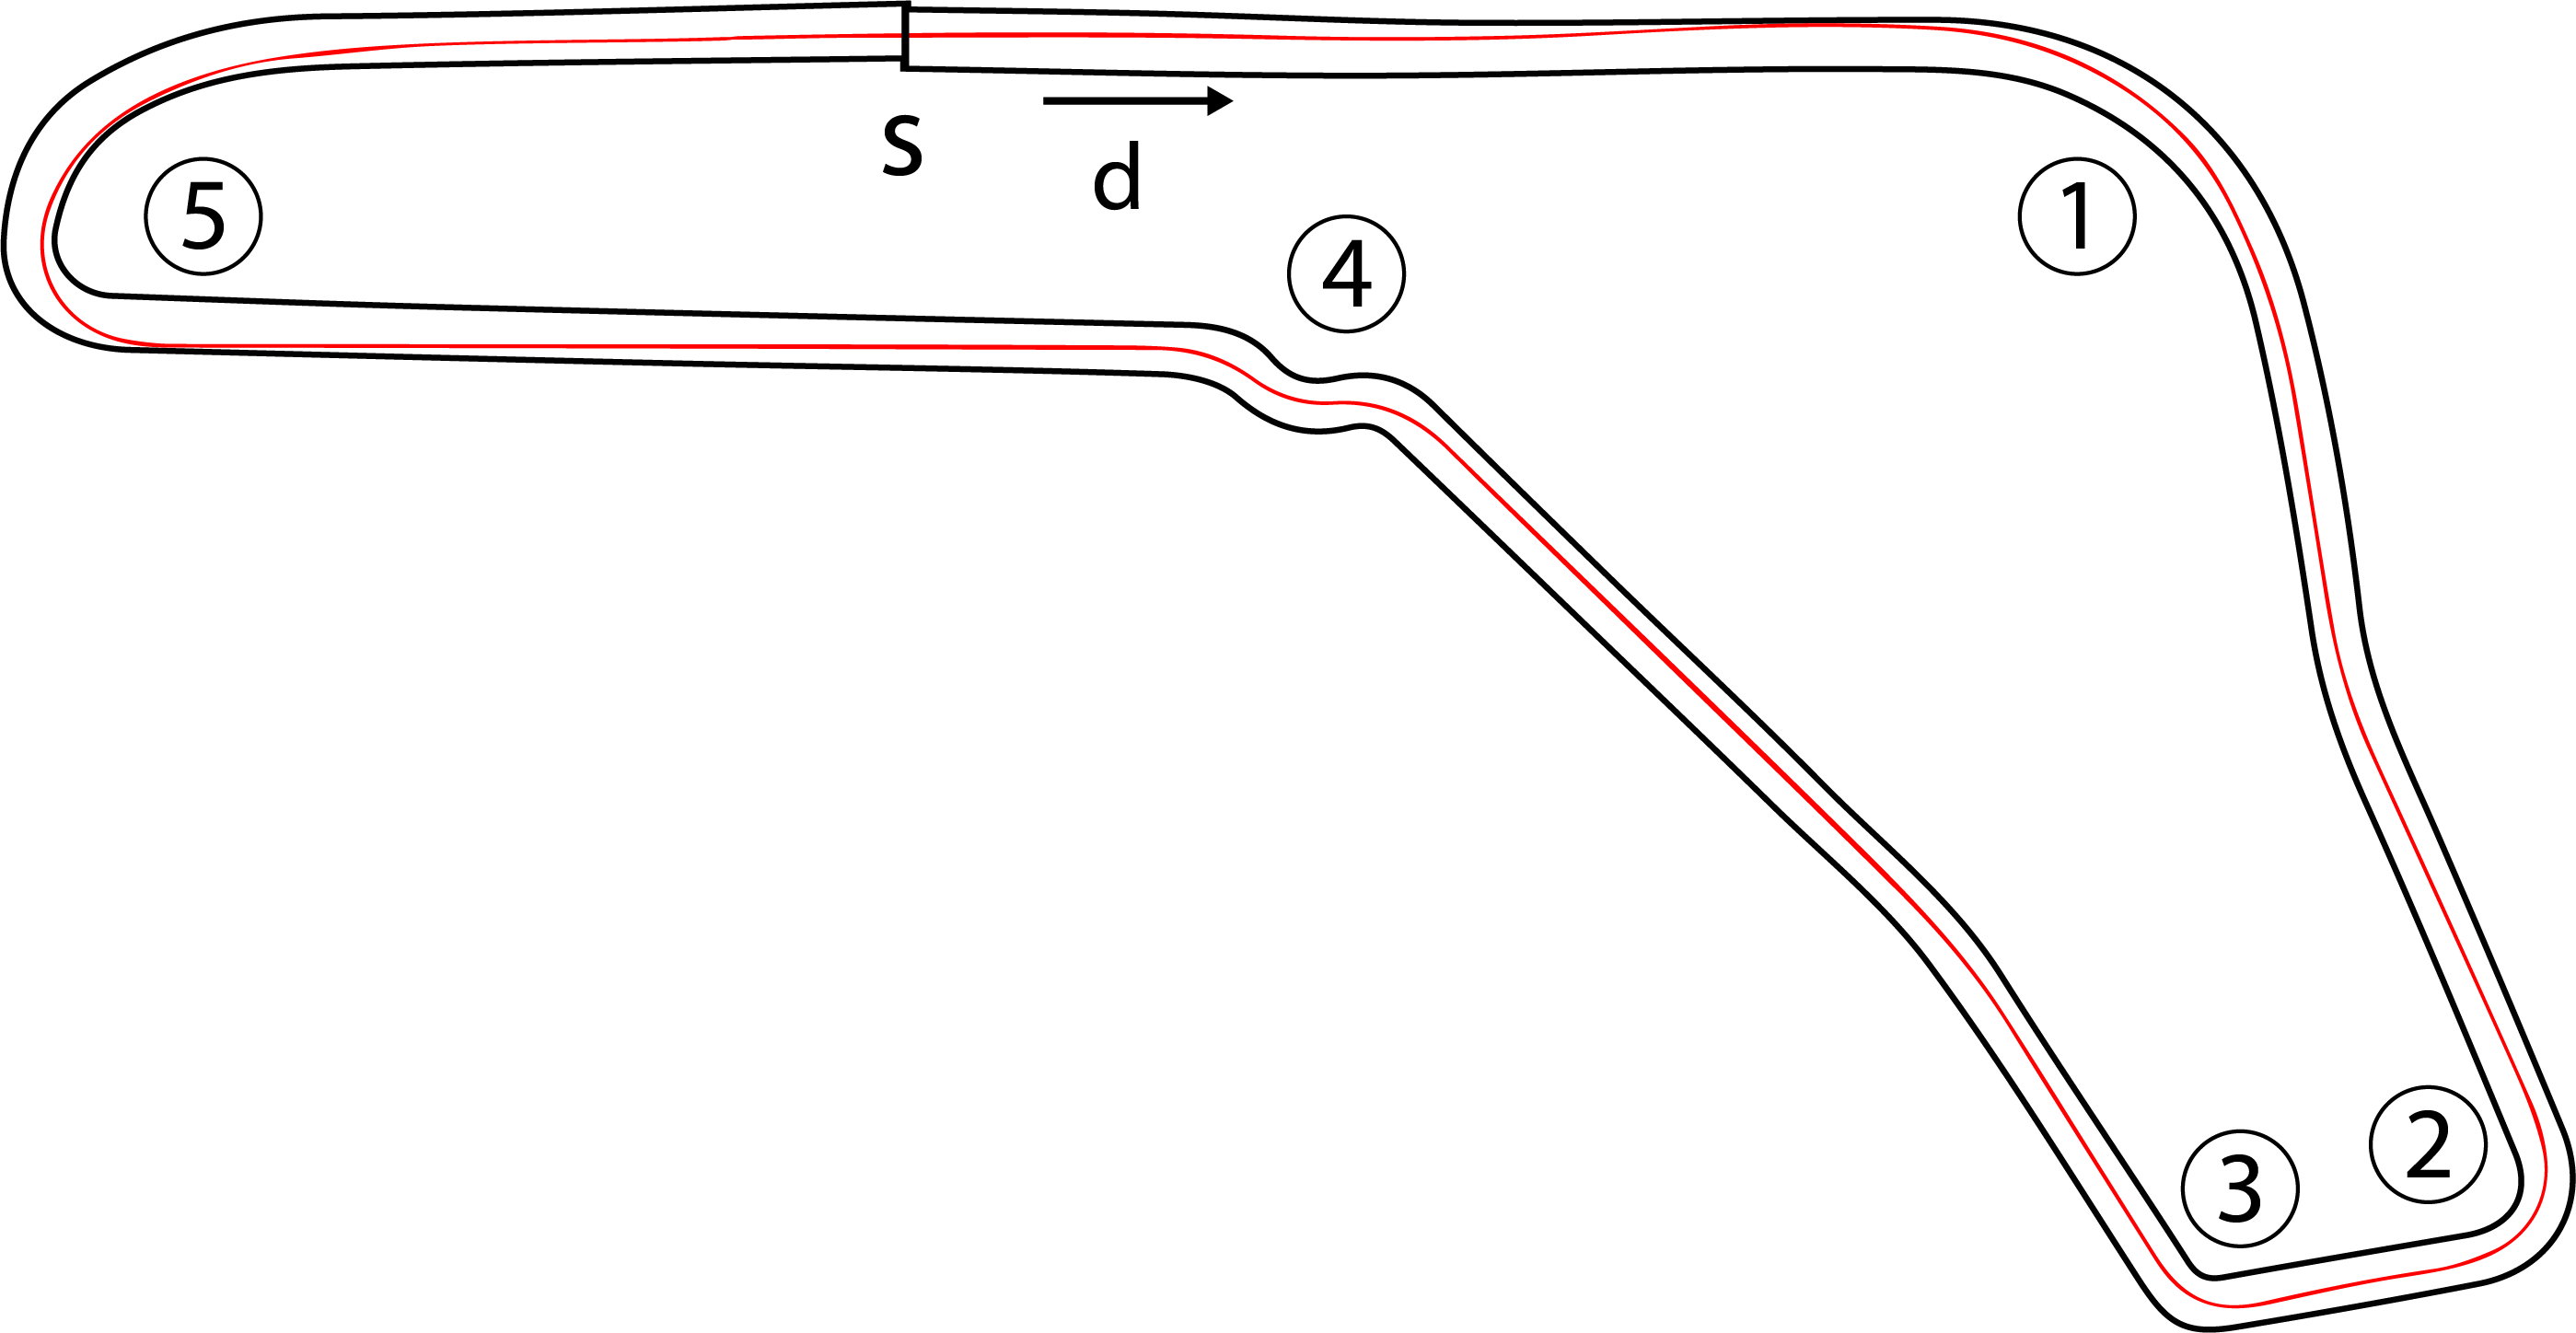
\includegraphics[width=12cm]{./img/ref_traj}
  \caption{Reference trajectory, where $s$ is the starting point and $d$ is the driving direction.}
   \label{fig:ref_traj}
\end{figure}

After the expert demonstrations are collected and the reference trajectory has been defined, it is possible to apply the algorithms described in Chatper \ref{Methods}. First of all, we discuss the two-step framework which consists in learning a policy
that follows the reference trajectory and another one that improves the lap time. This framework is formulated in Sections \ref{ref_follow}, and \ref{ref_improve} for policy following and improvement respectively. Then, we will discuss about the direct approach which consists in learning a single policy that learns to drive by using human demonstrations.

In the next sections, we will show the results obtained for each algorithm.

\section{Two-step Framework}
As described in Chapter 5, for the two step framework we used the algorithms POIS for the first stage and PPO for the second one. Before to apply POIS on the controller we inizialied the controller parameters $\boldsymbol {\omega}_0$ manually with a trial and error approach. This is done to speed up the initial learning phase of the algorithms, indeed, we run POIS over a set of controller's parameters that allows the controller to complete a lap.
Even if the human-initialized controller was able to complete a lap, it has the main limitation that the car during tight curves goes a bit out of track. As we will see, the optimization made by the RL algorithm is able to solve
this issue.

In this section, we will show the result of the optimization policy via POIS and of the obtained estimation of the optimal rule-based policy $\psi^*_{\boldsymbol \omega}$ , i.e. $\hat{\psi^*}_{\boldsymbol \omega}$.
\subsection{POIS}
We run POIS with the parameter vector $\boldsymbol {\omega}_0$ shown in Table \ref{tab:omega_0}. Every iteration consists in a batch of $200$ trajectories. Since the the environment is deterministic, each trajectory is obtained by sampling from the hyper-policy a parameter vector for each trajectory. The reward function we used is $r_{\text{space}}$ (Eq. \ref{eq:r_space}). In order to avoid the agent to go out of track we used a negative penalty equal to $-2000$ that is added to the reward signal. Figure \ref{fig:poislearning} depicts the mean reward of the $200$ trajectories: on the $x$ axis we have the iterations made by the algorithm, on the $y$ is the reward function. From this plot we notice that the algorithm converges around $8000$ iterations.

\begin{table}[H]

\centering
\begin{tabular}{|c|c|}
\hline
\textbf{$\boldsymbol {\omega}_0^i$} & \textbf{Value} \\ \hline
$\alpha_1$         & 0.5            \\ \hline
$\alpha_2$         & 0.02           \\ \hline
$\alpha_3$         & 5              \\ \hline
$\beta_1$          & 0.055          \\ \hline
$\gamma_1$         & 3          \\ \hline
$\gamma_2$         & 73.5          \\ \hline
$\gamma_3$         & 116          \\ \hline


\end{tabular}
\caption{Hand-tuned initialization of $\boldsymbol {\omega}_0$}
\label{tab:omega_0}
\end{table}




\begin{figure}[H]
\hspace*{-1cm}
 \centering
  \captionsetup{width=12cm}
  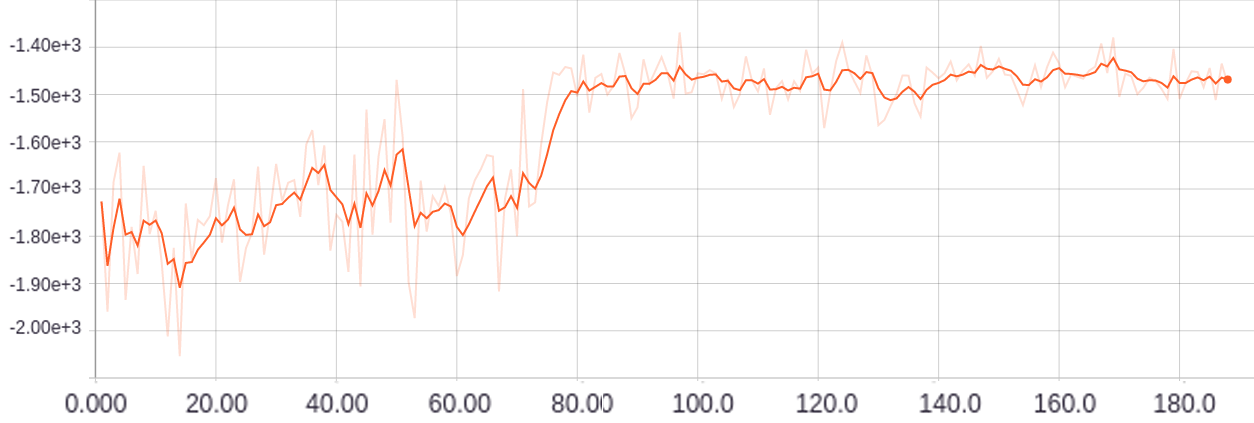
\includegraphics[width=14cm]{./img/optimiz}
  \caption{POIS optimization progress. On the $x$ axis is the number of iterations, on the $y$ axis is the mean value of the reward function for the sampled trajectories}
   \label{fig:poislearning}
\end{figure}

Fig.\ref{fig:means} and Fig.\ref{fig:means2} show the optimization progress of the hyperpolicy $\nu_{\boldsymbol \rho}$ with respect to the amount of sampled trajectory.
That is, Fig.\ref{fig:means} shows the learning progress of $\boldsymbol \omega$, which is the mean value of the parameter $\boldsymbol \rho$.
Fig.\ref{fig:means2} shows with a higher level of detail the progress of the means parameters $\alpha_1$,$\alpha_2$,$\alpha_3$, $\beta_1$, $\gamma_1$, which in Fig.\ref{fig:means} are too skewed to appreciate the differences.
The parameter $\boldsymbol \omega$ has been initialized with a vector $\boldsymbol \omega_0$ found with a trial-and-error approach.

\begin{figure}[H]
 \centering
  \captionsetup{width=10cm}
  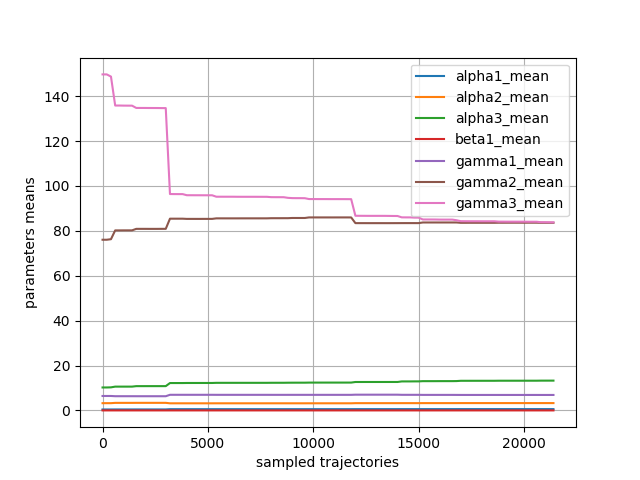
\includegraphics[width=10cm]{./img/parameters/means1}
  \caption{On the $x$ axis is the number of sampled trajectories; on the $y$ axis is the mean value of each parameter $\omega_i$}
   \label{fig:means}
\end{figure}

\begin{figure}[H]
 \centering
  \captionsetup{width=10cm}
  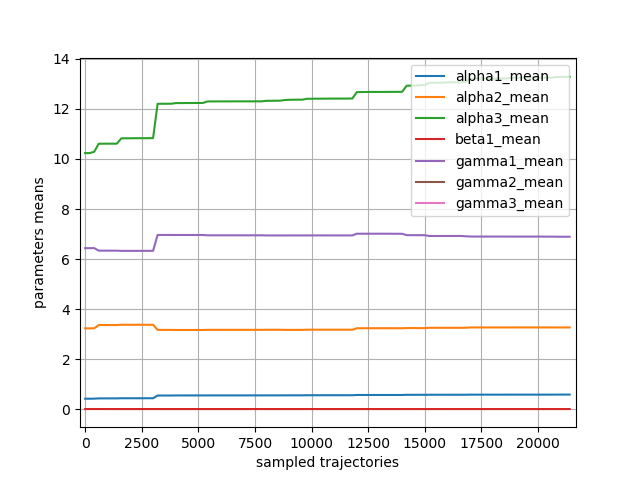
\includegraphics[width=10cm]{./img/parameters/means2}
  \caption{On the $x$ axis is the amount of sampled trajectories; on the $y$ axis is the mean value of each parameter $\omega_i$}
   \label{fig:means2}
\end{figure}


Fig.\ref{fig:log_stds} shows the progress of the standard deviations $\boldsymbol \sigma$. For a better visualization, we plotted the natural logarithm of the standard deviation instead of the std.
The parameter $\boldsymbol \sigma$ has been initialized with a vector $\boldsymbol \sigma_0= \boldsymbol 1.$ As expected, the standard deviations, as the number of sampled trajectories grow, tend to decrease. This means that the algorithm tends to explore less and less.


\begin{figure}[H]
 \centering
  \captionsetup{width=10cm}
  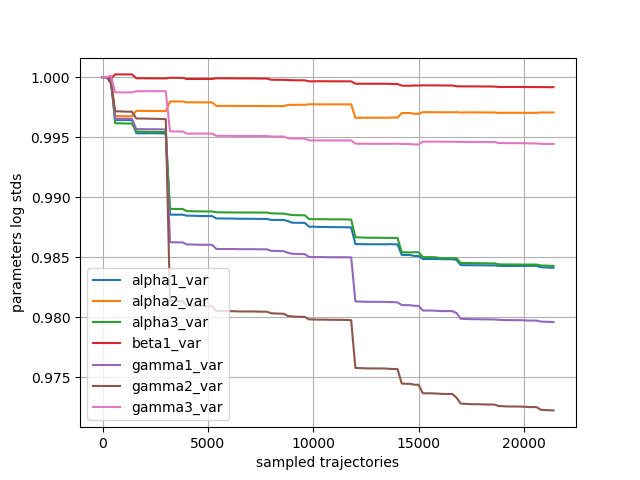
\includegraphics[width=10cm]{./img/parameters/log_stds}
  \caption{On the $x$ axis is the amount of sampled trajectories; on the $y$ axis is the logarithm of the standard deviation of each parameter $\omega_i$}
   \label{fig:log_stds}
\end{figure}



\subsubsection{Delta analysis}

The purpose of the rule-based policy $\psi_{\boldsymbol \omega}$ is to follow the reference trajectory. This translates into minimizing the difference between their position, velocity and orientation.
What follows shows the behavior of the optimal controller obtained by being trained with POIS, compared to the one fed with hand-tuned parameters, with respect to the reference trajectory.

\textbf{Delta position}
\label{sec:deltarho}
Fig.\ref{fig:delta_position} shows a comparison between the delta of the positions (i.e. the Euclidean distance) with respect to the reference trajectory along it, of the human-coded controller and the learned one.
As it can be noticed, the learned controller is almost always closer in the domain space to the reference trajectory with respect to the human one.

\begin{figure}[H]
 \centering
  \captionsetup{width=10cm}
  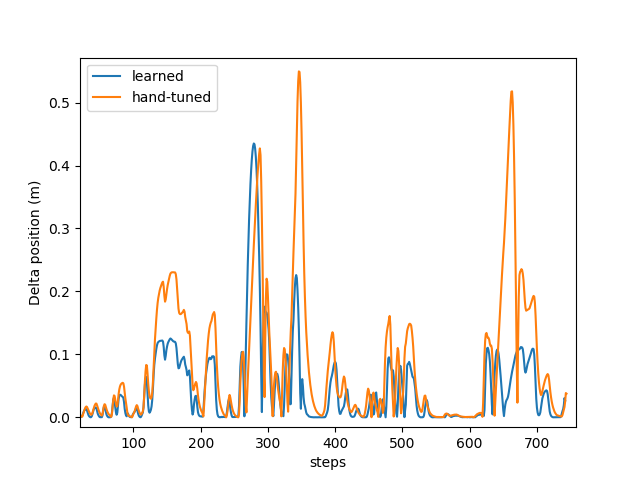
\includegraphics[width=10cm]{./img/deltas_pois/delta_position}
  \caption{On the $x$ axis are the steps of the trajectories, on the $y$ are the delta position, i.e. the 2D Euclidean distances between the reference trajectory and the two version of the controller.}
   \label{fig:delta_position}
 
Fig.\ref{fig:deltaposexpl} shows a detail of the comparison between the trajectories generated by the controller with human-crafted features and with a POIS learned policy with respect to the curves number 3 and 5. It can be noticed that in both these two curves the learned policy outperforms the hand-tuned one, following the reference trajectory with a higher level of accuracy.
 
\end{figure}
\begin{figure}[H]
\centering
\subfigure[Curve 3]
{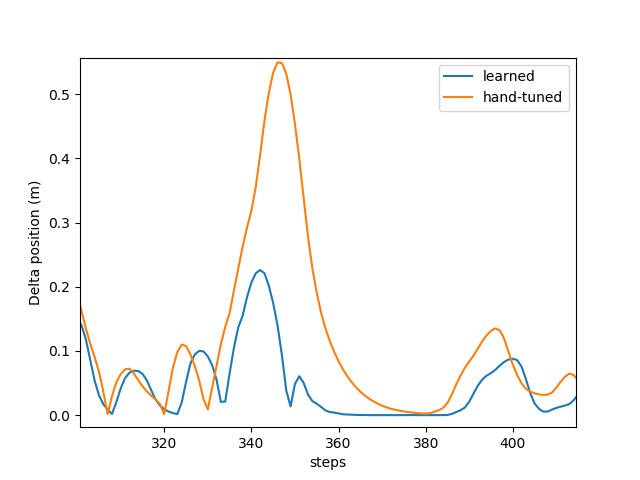
\includegraphics[width=6cm]{./img//deltas_pois/delta_rho_curva3}}
\hspace{3mm}
\subfigure[Curve 5]
{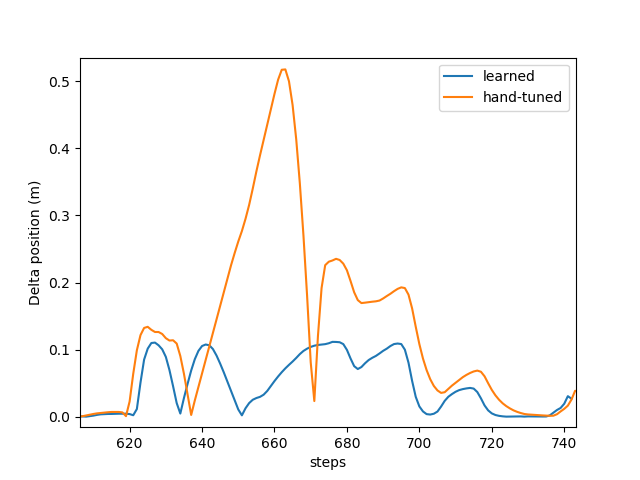
\includegraphics[width=6cm]{./img/deltas_pois/delta_rho_curva5}}
\caption{Detail of curves 3 and 5, with the comparison between the hand-tuned policy parameters and the learned policy parameters with respect to the reference trajectory concerning the position.}
\label{fig:deltaposexpl}
\end{figure}

In Fig.\ref{fig:curvespos}, this behaviour is show from the perspective of the absolute coordinates $(x,y)$.




\begin{figure}[H]
\centering
\subfigure[Curve 3]
{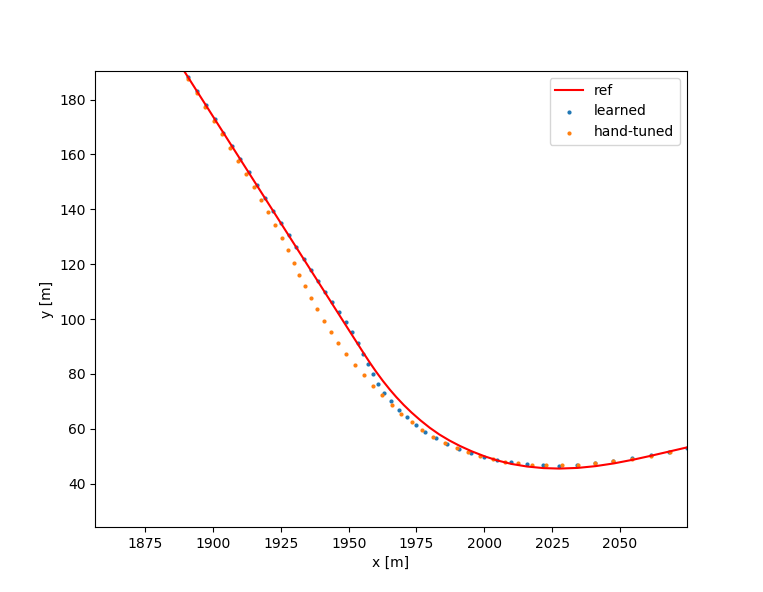
\includegraphics[width=7cm]{./img/traj_map/curve3}}
\hspace{2mm}
\subfigure[Curve 5]
{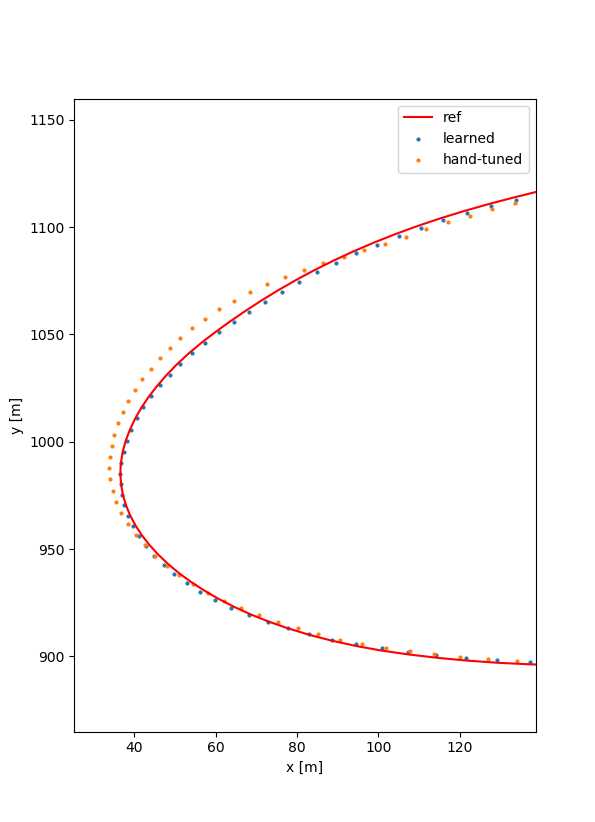
\includegraphics[width=5cm]{./img/traj_map/curve5}}
\caption{Detail of curves 3 and 5, with the comparison between the hand-tuned policy parameters and the learned policy parameters with respect to the reference trajectory, regarding the coordinates $(x,y)$.}
\label{fig:curvespos}
\end{figure}





\textbf{Delta velocity}
What follows are the results of the minimization of the difference of the rule-based policy and the reference trajectory concerning the speed. In particular, we focus on the longitudinal velocity, which is more meaningful for the lap-time metrics.
In Fig.\ref{fig:delta_vx} is represented the difference between the longitudinal velocities of the learned and human controller with respect with the reference trajectory. In Fig.\ref{fig:deltavxexpl} are the details on the curve 2 and 5.


\begin{figure}[H]
 \centering
  \captionsetup{width=10cm}
  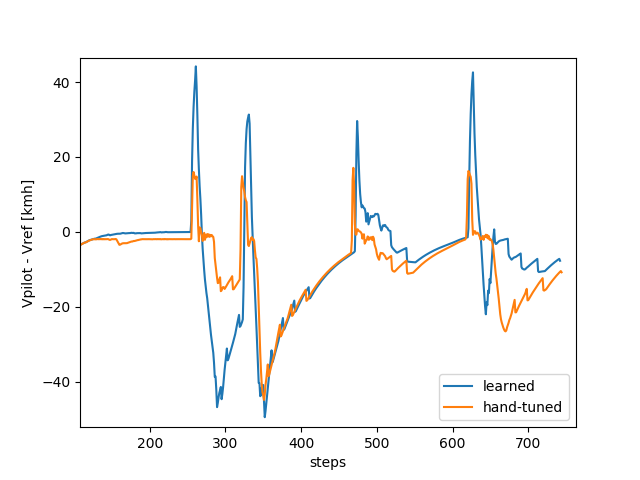
\includegraphics[width=10cm]{./img/deltas_pois/delta_vx}
  \caption{Full lap plot of the speed along the reference trajectory, the learned policy and the hand-tuned parameters.  On the $x$ axis are the trajectory steps; on the $y$ axis is the speed of the car.}
   \label{fig:delta_vx}
\end{figure}

\begin{figure}[H]
\centering
\subfigure[Curve 2]
{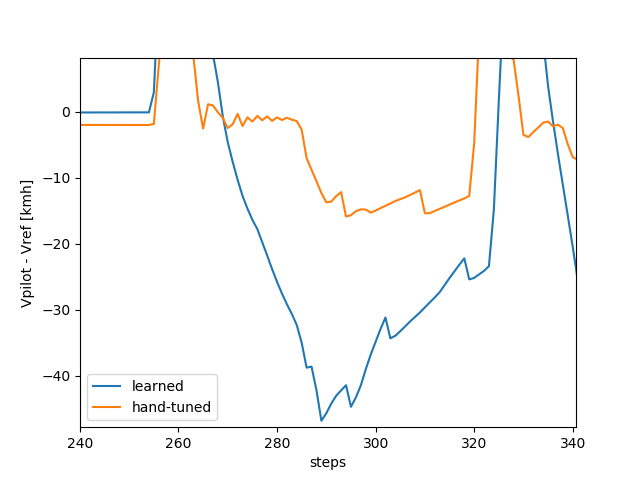
\includegraphics[width=6cm]{./img/deltas_pois/delta_vx_curva2}}
\hspace{3mm}
\subfigure[Curve 5]
{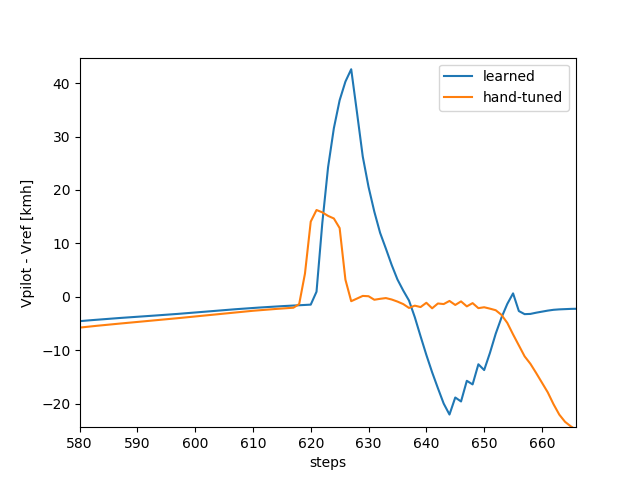
\includegraphics[width=6cm]{./img/deltas_pois/delta_vx_curva5}}
\caption{Comparisons of the differences of the longitudinal velocities between the reference trajectory and two policies: one with the learned parameters, the other with the hand-tuned parameters. On the $x$ axis are the trajectory steps; on the $y$ axis is the longitudinal velocities.}
\label{fig:deltavxexpl}
\end{figure}


Fig.\ref{fig:Vx} shows the behaviour of the policy from the point of view of the longitudinal velocity $v_x$.
In particular, Fig.\ref{fig:vxexpl} shows in detail the behaviors in curve 2 and 5 with respect to the reference trajectory regarding the speed. These behaviors especially occur in the curves, where the controller with the learned parameters runs at a lower speed with respect to the hand-tuned parameters. This behavior results effective for better following the reference trajectory position. In fact, as it can be seen in Table \ref{tab:avgspeed}, the average speeds of the learned parameters policy is slightly better than the hand-tuned one, because the lower speed on the corners allows to travel a lower distance, as also seen in Section \ref{sec:deltarho}

\begin{figure}[H]
 \centering
  \captionsetup{width=10cm}
  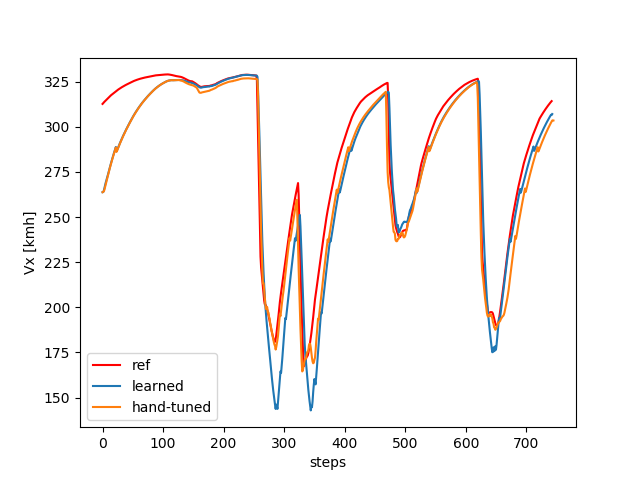
\includegraphics[width=10cm]{./img/velocities_pois/speed_x_comparison}
  \caption{On the $x$ axis are the steps of the trajectories, on the $y$ delta of the longitudinal velocity of human and learned controller with respect to the reference trajectory.}
   \label{fig:Vx}
\end{figure}

\begin{figure}[H]
\centering
\subfigure[Curve 2]
{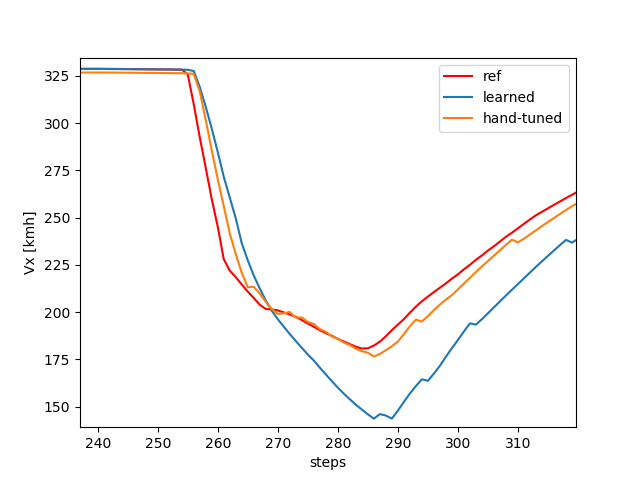
\includegraphics[width=6cm]{./img/velocities_pois/vx_curva2}}
\hspace{3mm}
\subfigure[Curve 5]
{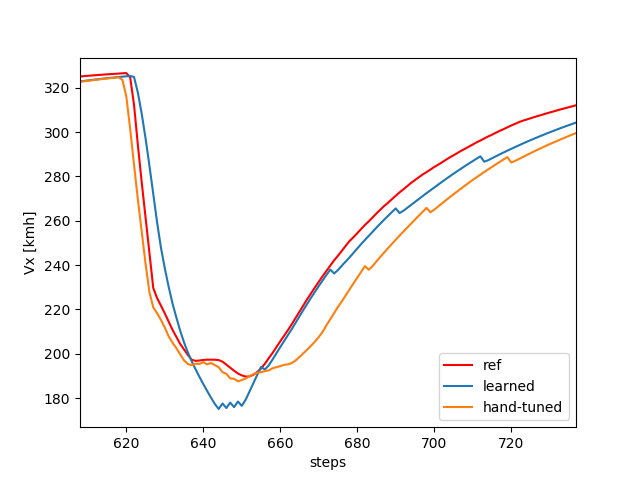
\includegraphics[width=6cm]{./img/velocities_pois/vx_curva5_rettilineo_finale}}
\caption{Detail of curves 2 and 5, with the comparison between the hand-tuned policy parameters and the learned policy parameters with respect to the reference trajectory concerning the longitudinal velocity.}
\label{fig:vxexpl}
\end{figure}

\begin{table}[H]
\centering
\begin{tabular}{|c|c|}
\hline
\textbf{Driver}                                                                      & \textbf{Average Lap-Speed (kmh)} \\ \hline
Reference  Trajectory   & 288.13                 \\ \hline
\begin{tabular}[c]{@{}c@{}}Controller\\  (Human Crafted Parameter)\end{tabular}      & 277.38                 \\
\hline
\begin{tabular}[c]{@{}c@{}}Controller\\  (Learned Parameters with POIS)\end{tabular} & 277.96     \\ \hline           
\end{tabular}
\caption{Average speed to complete a lap.}
\label{tab:avgspeed}
\end{table}

\textbf{Delta Orientation}

In Fig. \ref{fig:deltaorien} we show the orientation differences of curve number 2 and 5. It can be noticed that the controller with the two different sets of parameters does not show big discrepancy, but in some cases it results been more stable.

\begin{figure}[H]
\centering
\subfigure[Curve 2]
{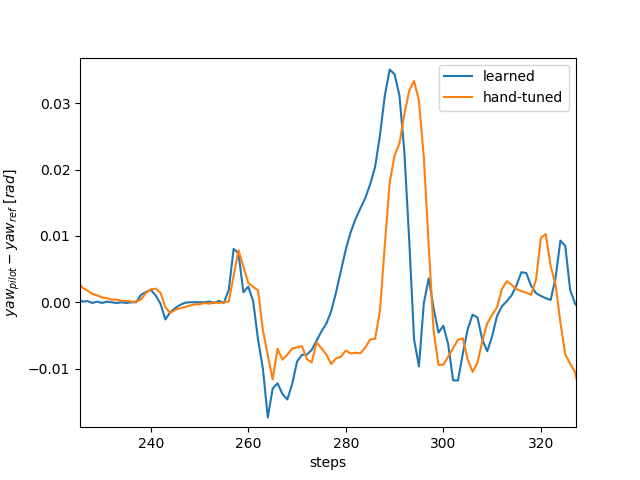
\includegraphics[width=6cm]{./img/deltas_pois/delta_orientation_curva2}}
\hspace{3mm}
\subfigure[Curve 5]
{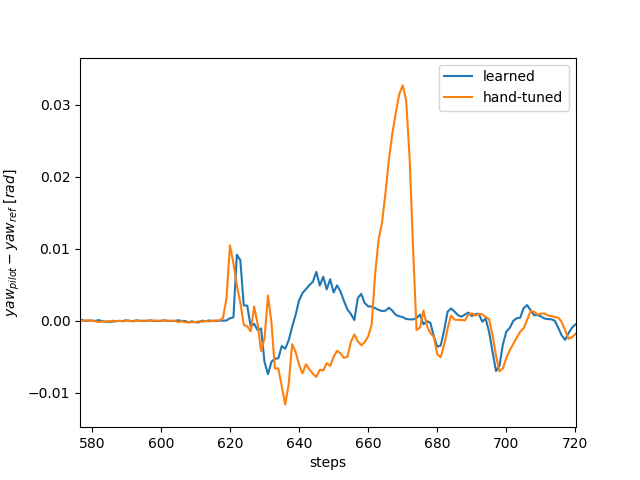
\includegraphics[width=6cm]{./img/deltas_pois/delta_orientation_curva5}}
\caption{Comparisons of the differences of orientations between the reference trajectory and two policies: one with the learned parameters, the other with the hand-tuned parameters. On the $x$ axis are the trajectory steps; on the $y$ axis is the delta orientation.}
\label{fig:deltaorien}
\end{figure}


In Fig.\ref{fig:laptime_pois} is shown the progress of the lap-time obtained with the rule-based policy $\psi_{\boldsymbol \omega}$ optimizing with POIS.
As expected, a rule-based policy itself cannot outperform the expert's performance. In fact, at converge, i.e. at the optimal delta minimization, not only it does not obtain a better lap-time with respect to the reference trajectory (see Table \ref{table:controller_lap_time}), but it is not even the best it obtains along its learning process.


\begin{figure}[H]
 \centering
  \captionsetup{width=10cm}
  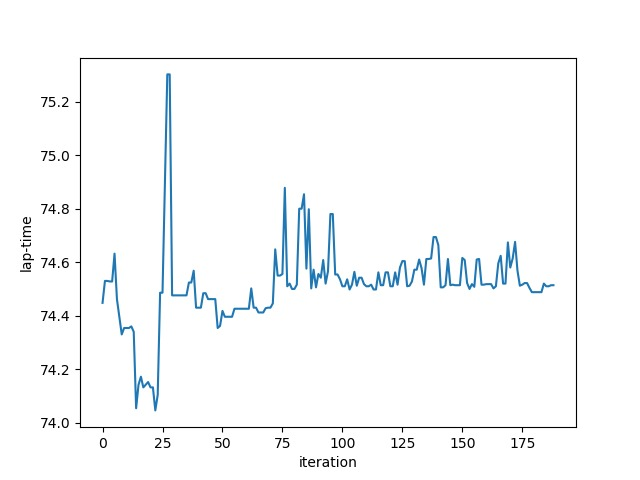
\includegraphics[width=10cm]{./img/means-lap-time}
  \caption{On the $x$ axis is the amount of sampled trajectories; on the $y$ axis is the logarithm of the standard deviation of each parameter $\omega_i$}
   \label{fig:laptime_pois}
\end{figure}





\begin{table}[H]
\centering
\begin{tabular}{|c|c|}
\hline
\textbf{Driver}                                                                      & \textbf{Lap-time (s)} \\ \hline
Reference  Trajectory   & 71.99                 \\ \hline
\begin{tabular}[c]{@{}c@{}}Controller\\  (Human Crafted Parameter)\end{tabular}      & 74.50                 \\
\hline
\begin{tabular}[c]{@{}c@{}}Controller\\  (Learned Parameters with POIS)\end{tabular} & 74.45     \\ \hline           
\end{tabular}
\caption{Best lap-time obtained by each algorithm with respect to the reference trajectory}
\label{table:controller_lap_time}
\end{table}


Concluding, the controller optimized with POIS behaves as expected, being able to follow the reference trajectory with a satisfying degree of accuracy.
However, it shows some deviating behaviours with respect to the reference trajectory regarding the speed. These behaviors especially occur in the curves, where the controller with the learned parameters runs at a lower speed with respect to the hand-tuned parameters. 


\section{Action Analysis}

\textbf{Throttle}
\begin{figure}[H]
 \centering
  \captionsetup{width=10cm}
  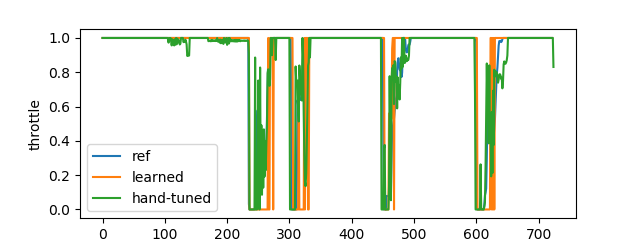
\includegraphics[width=10cm]{./img/action_pois/throttle}
  \caption{On the $x$ axis are the steps of the trajectories, on the $y$ delta of the longitudinal velocity of human and learned controller with respect to the reference trajectory.}
   \label{fig:throttle}
\end{figure}

\begin{figure}[H]
\centering
\subfigure[Curve 2]
{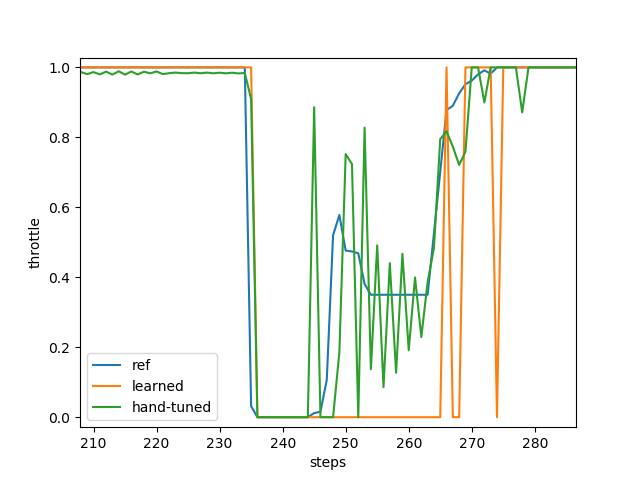
\includegraphics[width=6cm]{./img/action_pois/throttle_curva2}}
\hspace{1mm}
\subfigure[Curve 3]
{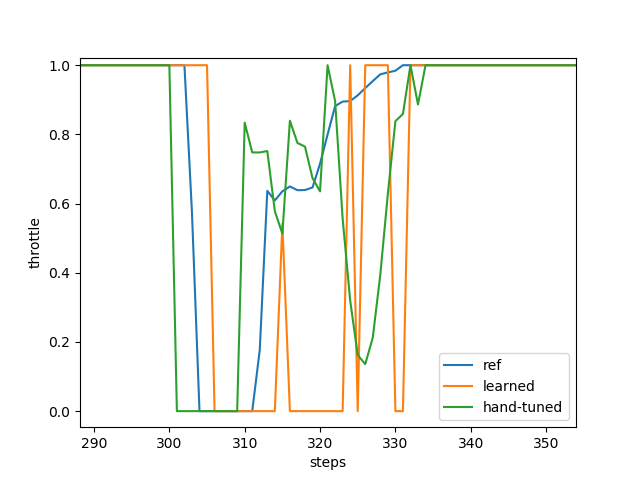
\includegraphics[width=6cm]{./img/action_pois/throttle_curva3}}
\hspace{1mm}
\subfigure[Curve 4]
{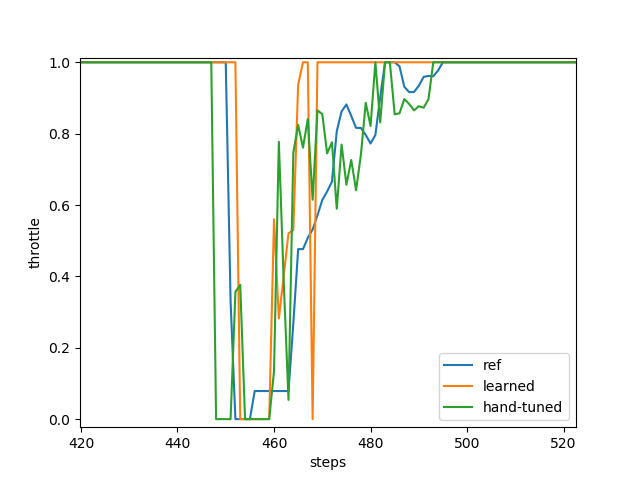
\includegraphics[width=6cm]{./img/action_pois/throttle_curva4}}
\hspace{1mm}
\subfigure[Curve 5]
{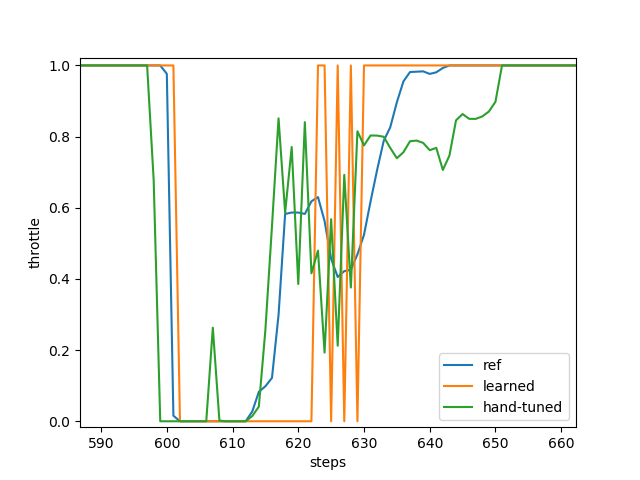
\includegraphics[width=6cm]{./img/action_pois/throttle_curva5}}
\caption{Comparisons of the differences of orientations between the reference trajectory and two policies: one with the learned parameters, the other with the hand-tuned parameters. On the $x$ axis are the trajectory steps; on the $y$ axis is the delta orientation.}
\label{fig:throttleexpl}
\end{figure}

\begin{figure}[H]
 \centering
  \captionsetup{width=10cm}
  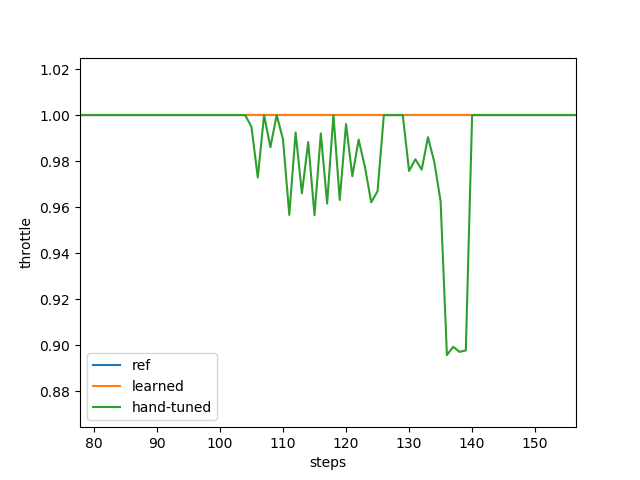
\includegraphics[width=10cm]{./img/action_pois/throttle_rettilineo}
  \caption{On the $x$ axis is the amount of sampled trajectories; on the $y$ axis is the logarithm of the standard deviation of each parameter $\omega_i$}
   \label{fig:throttleexplrett}
\end{figure}





\textbf{Brake}
\begin{figure}[H]
\hspace*{-1cm}
 \centering
  \captionsetup{width=10cm}
  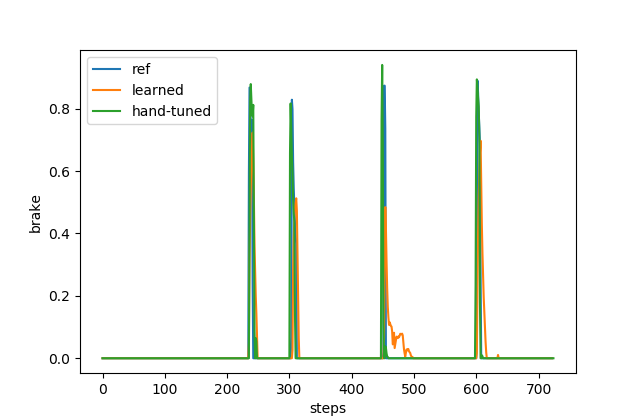
\includegraphics[width=10cm]{./img/action_pois/brake}
  \caption{On the $x$ axis are the steps of the trajectories, on the $y$ delta of the longitudinal velocity of human and learned controller with respect to the reference trajectory.}
   \label{fig:brake}
\end{figure}

\begin{figure}[H]
\centering
\subfigure[Curve 2]
{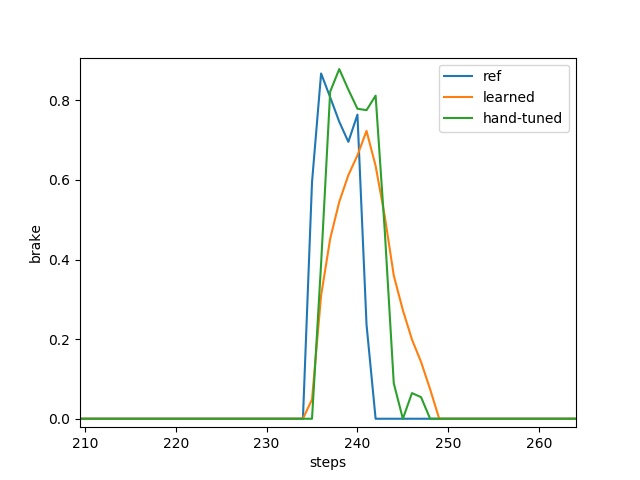
\includegraphics[width=6cm]{./img/action_pois/brake_human_curva2}}
\hspace{1mm}
\subfigure[Curve 3]
{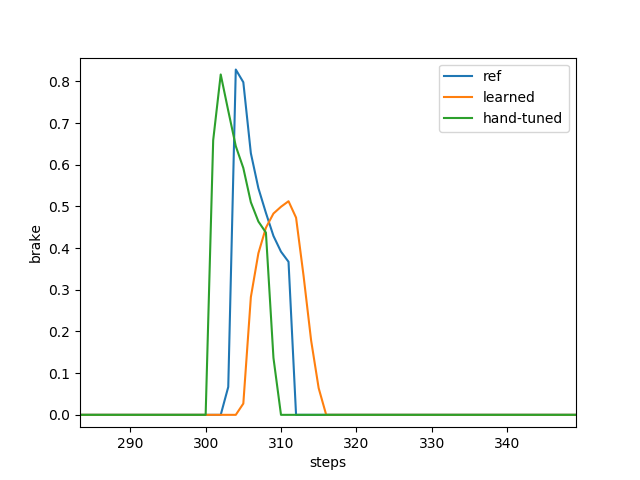
\includegraphics[width=6cm]{./img/action_pois/brake_human_curva3}}
\hspace{1mm}
\subfigure[Curve 4]
{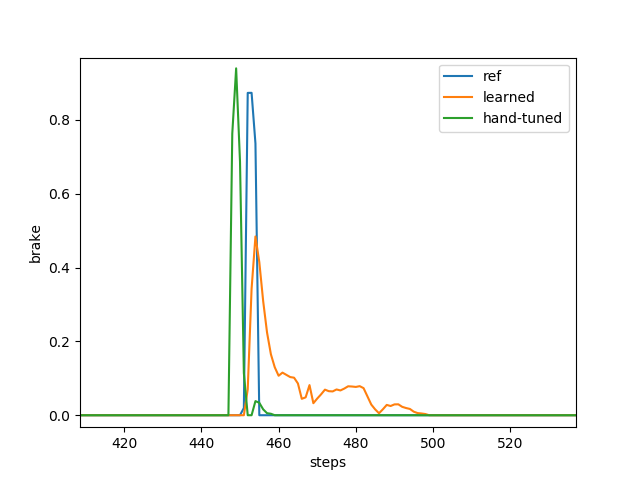
\includegraphics[width=6cm]{./img/action_pois/brake_human_curva4}}
\hspace{1mm}
\subfigure[Curve 5]
{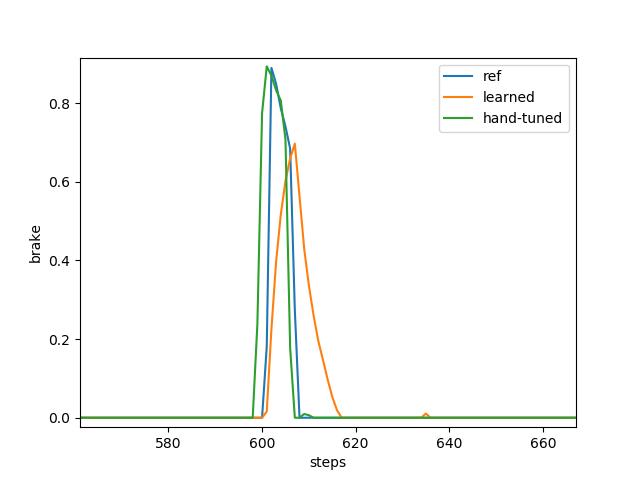
\includegraphics[width=6cm]{./img/action_pois/brake_human_curva5}}
\caption{Comparisons of the differences of orientations between the reference trajectory and two policies: one with the learned parameters, the other with the hand-tuned parameters. On the $x$ axis are the trajectory steps; on the $y$ axis is the delta orientation.}
\label{fig:brakeexpl}
\end{figure}


\textbf{Steer}
\begin{figure}[H]
 \centering
  \captionsetup{width=10cm}
  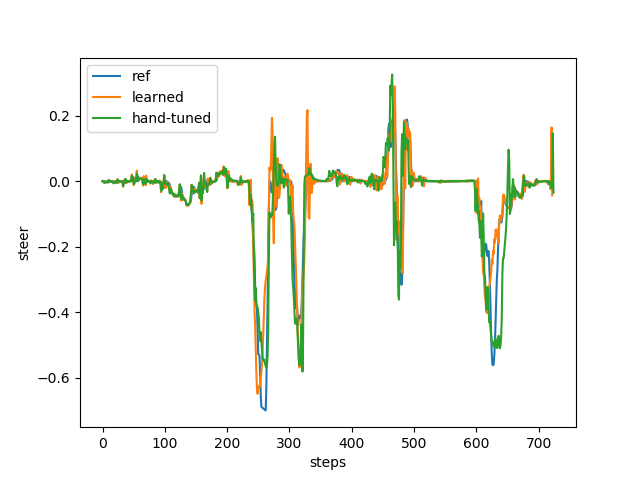
\includegraphics[width=10cm]{./img/action_pois/steer}
  \caption{On the $x$ axis are the steps of the trajectories, on the $y$ delta of the longitudinal velocity of human and learned controller with respect to the reference trajectory.}
   \label{fig:steer}
\end{figure}





\subsection{PPO}






\chapter{Experiments}
\label{Experiments}
\thispagestyle{empty}

TESTO CAPITOLO 7
\chapter{Conclusion}
\label{Conclusion}
\thispagestyle{empty}

TESTO CAPITOLO 8

\cleardoublepage

% ---- Bibliography ----
\addcontentsline{toc}{chapter}{Bibliography}
\bibliographystyle{plain}
\bibliography{bibl_thesis}
\appendix

%\pagestyle{fancy} 
%\fancyfoot{}                                               
%\renewcommand{\chaptermark}[1]{\markboth{\appendixname\ \thechapter.\ #1}{}} 
%\renewcommand{\sectionmark}[1]{\markright{\thesection.\ #1}}         
%\fancyhead[LE,RO]{\bfseries\thepage}    
%                                        
%\fancyhead[RE]{\bfseries\leftmark}    
%\fancyhead[LO]{\bfseries\rightmark}     
%\renewcommand{\headrulewidth}{0.3pt} 

%\include{appendices/appendixA}


\end{document}